% example for dissertation.sty
\documentclass[
  % Replace oneside by twoside if you are printing your thesis on both sides
  % of the paper, leave as is for single sided prints or for viewing on screen.
  oneside,
  %twoside,
  11pt, a4paper,
  footinclude=true,
  cleardoublepage=empty
]{scrbook}

\usepackage{dissertation}
\usepackage[english]{babel}
\usepackage[utf8]{inputenc}
\usepackage{amsmath}
\usepackage{algorithm}
\usepackage[noend]{algpseudocode}
\setcounter{secnumdepth}{3}
%\setcounter{tocdepth}{3}
\usepackage{pgfplots}
\usepackage{csquotes}
\usepackage{indentfirst}
\usepackage{listings}
\usepackage{color}
\usepackage[
    type={CC},
    modifier={by},
    version={4.0},
]{doclicense}
\usepackage{afterpage}
\newcommand\myemptypage{
\null
\thispagestyle{empty}
\addtocounter{page}{-1}
\newpage
}
\usepackage[T1]{fontenc}
\lstset{
upquote=true,
literate=
{á}{{\'a}}1 {é}{{\'e}}1 {í}{{\'i}}1 {ó}{{\'o}}1 {ú}{{\'u}}1
{Á}{{\'A}}1 {É}{{\'E}}1 {Í}{{\'I}}1 {Ó}{{\'O}}1 {Ú}{{\'U}}1
{à}{{\`a}}1 {è}{{\`e}}1 {ì}{{\`i}}1 {ò}{{\`o}}1 {ù}{{\`u}}1
{À}{{\`A}}1 {È}{{\'E}}1 {Ì}{{\`I}}1 {Ò}{{\`O}}1 {Ù}{{\`U}}1
{ä}{{\"a}}1 {ë}{{\"e}}1 {ï}{{\"i}}1 {ö}{{\"o}}1 {ü}{{\"u}}1
{Ä}{{\"A}}1 {Ë}{{\"E}}1 {Ï}{{\"I}}1 {Ö}{{\"O}}1 {Ü}{{\"U}}1
{â}{{\^a}}1 {ê}{{\^e}}1 {î}{{\^i}}1 {ô}{{\^o}}1 {û}{{\^u}}1
{Â}{{\^A}}1 {Ê}{{\^E}}1 {Î}{{\^I}}1 {Ô}{{\^O}}1 {Û}{{\^U}}1
{ã}{{\~a}}1 {ẽ}{{\~e}}1 {ĩ}{{\~i}}1 {õ}{{\~o}}1 {ũ}{{\~u}}1
{Ã}{{\~A}}1 {Ẽ}{{\~E}}1 {Ĩ}{{\~I}}1 {Õ}{{\~O}}1 {Ũ}{{\~U}}1
{œ}{{\oe}}1 {Œ}{{\OE}}1 {æ}{{\ae}}1 {Æ}{{\AE}}1 {ß}{{\ss}}1
{ű}{{\H{u}}}1 {Ű}{{\H{U}}}1 {ő}{{\H{o}}}1 {Ő}{{\H{O}}}1
{ç}{{\c c}}1 {Ç}{{\c C}}1 {ø}{{\o}}1 {å}{{\r a}}1 {Å}{{\r A}}1
{€}{{\euro}}1 {£}{{\pounds}}1 {«}{{\guillemotleft}}1
{»}{{\guillemotright}}1 {ñ}{{\~n}}1 {Ñ}{{\~N}}1 {¿}{{?`}}1 {¡}{{!`}}1
}

% \newcommand{\SYS}{H2Dedup\xspace}

\usepackage{amssymb}
\usepackage{enumitem}
\usepackage{environ}

\newcommand{\addnoteauthor}[2]{%
  \expandafter\newcommand\csname #1\endcsname[1]{%
    {%
      \small\color{black}%
      \fbox{\scriptsize\bfseries\sffamily#1}%
      $\blacktriangleright${\sffamily\itshape\color{#2}##1}$\blacktriangleleft$%
      }%
    }%
  \NewEnviron{#1block}{%
    \vspace*{.4\baselineskip}%
    \small\color{black}%
    \setlength\parskip{0pt plus 0pt minus 0pt}%
    \par\noindent\fbox{\scriptsize\bfseries\sffamily#1}%
    \par\nopagebreak\noindent\sffamily\itshape\color{#2}%
    \begin{tabularx}{\linewidth}{|X|}%
      \hline%
      \vspace{-2pt}%
      \BODY%
      \par \kern-6pt%
      \tabularnewline \hline%
    \end{tabularx}%
    \vspace*{.4\baselineskip}%
    }%
  \NewEnviron{#1itemize}{%
    \vspace*{.4\baselineskip}%
    \small\color{black}%
    \setlength\parskip{0pt plus 0pt minus 0pt}%
    \par\noindent\fbox{\scriptsize\bfseries\sffamily#1}%
    \par\nopagebreak\noindent\sffamily\itshape\color{#2}%
    \setlist{leftmargin=*,topsep=0pt,nosep}%
    \begin{tabularx}{\linewidth}{|X|}%
      \hline%
      \vspace{-2pt}%
      \begin{itemize}%
        \BODY%
      \end{itemize}%
      \par \kern-8pt%
      \tabularnewline \hline%
    \end{tabularx}%
    \vspace*{.4\baselineskip}%
    }%
  }

% \addnoteauthor{jtpaulo}{red}

% ACRONYMS -----------------------------------------------------

%import the necessary package with some options
\usepackage[acronym,nonumberlist,nomain]{glossaries}

%enable the following to avoid links from the acronym usage to the list
%\glsdisablehyper

%displays the first use of an acronym in italic
\defglsdisplayfirst[\acronymtype]{\emph{#1#4}}

%the style of the Glossary
\glossarystyle{list}

% set the name for the acronym entries page
\renewcommand{\glossaryname}{Acronyms}

%this shall be the last thing in the acronym configuration!!
\makeglossaries

% these could go in an acronyms.tex file, and loaded with:
% \loadglsentries[\acronymtype]{Parts/Definitions/acronyms}
% when using this, you may want to remove 'nomain' from the package options

%% **MORE INFO** %%

%to add the acronyms list add the following where you want to print it:
%\printglossary[type=\acronymtype]
%\clearpage
%\thispagestyle{empty}

%to use an acronym:
%\gls{qps}

% compile the thesis in command line with the following command sequence:
% pdlatex dissertation.tex
% makeglossaries dissertation
% bibtex dissertation
% pdlatex dissertation.tex
% pdlatex dissertation.tex

% ----------------------------------------------------------------

% Title
% Hybrid Inline and Offline Deduplication System
\titleA{Applying Attribute Grammars to teach Linguistic}
\titleB{Rules}
% \subtitleA{First Part of Subtitle}
% \subtitleB{Second part of Subtitle} % (if any)

% Author
\author{Manuel Gouveia Carneiro de Sousa}

% Supervisor(s)
\supervisor{Ph.D Pedro M. Rangel S. Henriques}
\cosupervisor{Ph.D Maria João T. Varanda Pereira}

% University (uncomment if you need to change default values)
% \def\school{Escola de Engenharia}
% \def\department{Departamento de Inform\'{a}tica}
% \def\university{Universidade do Minho}
% \def\masterdegree{Computer Science}

% Date
\date{\myear} % change to text if date is not today
% \date{June 2021}

% Keywords
%\keywords{master thesis}

% Glossaries & Acronyms
%\makeglossaries  %  either use this ...
%\makeindex	   % ... or this

% Define Acronyms
% Acronyms
\newacronym{DSL}{DSL}{Domain Specific Language}
\newacronym{ANTLR}{ANTLR}{Another Tool for Language Recognition}
\newacronym{CFG}{CFG}{Context-free Grammar}
\newacronym{AG}{AG}{Attribute Grammar}
\glsaddall[types={\acronymtype}]

\ummetadata % add metadata to the document (author, publisher, ...)

\begin{document}
	%%%%%%%%%%%%%%%%%%%%%% Cover Pages %%%%%%%%%%%%%%%%%%%%%%
	\umfrontcover	
	\umtitlepage
	
\myemptypage
    
	%%%%%%%%%%%%%%%%%%%%%%% Copyright %%%%%%%%%%%%%%%%%%%%%%%
	\chapter*{AUTHOR COPYRIGHTS AND TERMS OF USAGE BY THIRD PARTIES}
	This is an academic work which can be utilized by third parties given that the rules and good practices internationally accepted, regarding author copyrights and related copyrights.

Therefore, the present work can be utilized according to the terms provided in the license bellow.

If the user needs permission to use the work in conditions not foreseen by the licensing indicated, the user should contact the author, through the RepositóriUM of University of Minho.\\[0.5cm]

\textbf{License provided to the users of this work}


\includegraphics[width=0.2\textwidth]{images/license.png}

\textbf{Attribution-NonCommercial}

\textbf{CC BY-NC}

https://creativecommons.org/licenses/by-nc/4.0/
	
	%%%%%%%%%%%%%%%%% Statement Of Integrity %%%%%%%%%%%%%%%%
	\chapter*{STATEMENT OF INTEGRITY}
	I hereby declare having conducted this academic work with integrity. I confirm that I have not used plagiarism or any form of undue use of information or falsification of results along the process leading to its elaboration.

I further declare that I have fully acknowledged the Code of Ethical Conduct of the University of Minho.\\[0.5cm]

\begin{flushright}
\begin{tabular}{@{}p{1.2in}}
Manuel Sousa \\
\hrulefill \\
\end{tabular}
\end{flushright}
	
\myemptypage
\myemptypage
	
	%%%%%%%%%%%%%%%%%%%% Acknowledgments %%%%%%%%%%%%%%%%%%%%
	\chapter*{Acknowledgments}
	Todo o trabalho desenvolvido não seria possível sem o apoio de um grupo muito especial de pessoas.
Dessa forma, gostaria de aproveitar este momento para dedicar algumas palavras àqueles que acompanharam de perto este percurso.

Em primeiro lugar, um agradecimento aos meus pais, Noémia e Vitor, aos meus avós, Olinda e Manuel,
e aos meus tios, Adília e Cândido, que me tornaram o que sou hoje,
que me acompanharam durante toda a minha vida, ajudando-me sempre a superar as diversas dificuldades 
e desafios que foram surgindo. Pela forma de como me educaram e cuidaram de mim, estando sempre ao meu lado.

A ti, Beatriz, pela constante força, apoio e carinho, em todos os momentos. Por nunca me teres deixado desistir 
ou deixar de acreditar, mostrando-me sempre que consigo concretizar os meus objetivos.

Ao meu amigo de sempre, Diogo, pela constante compreensão e paciência para ouvir as minhas preocupações.
Por todos os momentos e por estar sempre presente.

Ao meu amigo Lázaro, por toda a sua motivação, dedicação e energia positiva. Pela sua constante preocupação com o meu percurso e por todas as oportunidades que me deu.

A todos os meus colegas que me acompanharam durante todo o percurso académico, cuja ajuda foi fulcral em todos os momentos.

Por último, aos meus orientadores, Professor Pedro Rangel Henriques e Professora Maria João Pereira, por todo o apoio, assistência e disponibilidade durante todo o processo e pela magnífica oportunidade que me foi dada, a minha especial gratidão.

\myemptypage
\myemptypage

	%%%%%%%%%%%%%%%%%%%%%%%% Abstract %%%%%%%%%%%%%%%%%%%%%%%
	% \cleardoublepage
	\chapter*{Abstract}
	This document presents the topic “Applying Attribute Grammars to teach Linguistic Rules”, at Universidade do Minho in Braga, Portugal.
This thesis is focused on using the formalisms of attribute grammars in order to create a tool to help linguistic students learn the different rules of a natural language. 
The system developed, named \textbf{Lyntax}, consists in a processor for a domain specific language which intends to enable the user to specify different kinds of
sentence structures, and afterwards, test various phrases against said structures.
The processor validates and evaluates the input given, generating a grammar which is specific to a previously chosen sentence.
Lastly, using \textsc{ANTLR}, a parser is generated for that specific grammar referred above. The processor built by \textsc{ANTLR} also creates a syntax tree that is presented to the user for analysis purposes.

An interface that supports the specification of the language (written in Lyntax DSL) was built, also allowing the use of the processor and the generation of the specific grammar,
exempting the user from knowing the details of the process.

Within this document, the focus will be primarly dedicated to the analysis of the system and how each block was built.
Different examples of the processor in action will be shown and explained.\\[0.1cm]

%The main goal is to create a new DSL with a simple notation,
%suitable for any person that does not have any experience with common programming languages elements, that will allow to define linguistic exercices. 
%Furthermore, it was created a user interface that supports that same tool, granting a more visual experience for the user.\\[0.1cm]

\noindent \textbf{Keywords}: Linguistic, Natural Language Processing, Attribute Grammar
	
	%%%%%%%%%%%%%%%%%%%%%%%%% Resumo %%%%%%%%%%%%%%%%%%%%%%%%
	\chapter*{Resumo}
	Este documento refere-se a uma dissertação sobre o tópico ``Aplicar Gramáticas de Atributos no ensino de Regras de Linguística'', 
e será concluída na Universidade do Minho em Braga, Portugal.
Esta dissertação pretende focar-se no uso dos formalismos das gramáticas de atributos de maneira a criar uma ferramenta que ajude os alunos de linguística a aprender 
as diversas regras da língua natural.

O sistema desenvolvido, denominado de \textbf{Lyntax}, consiste em um processor para uma linguagem de domínio específico cujo objetivo é o de permitir ao seu utilizador
a possibilidade de especificar diversas estruturas de frases, e posteriormente, testar frases contra essas mesmas estruturas.
O processador valida e avalia o input recebido, gerando uma gramática específica à frase previamente escolhida.
Por fim, usando uma ferramenta como o \textsc{ANTLR}, um parser é gerado para a gramática específica acima referida. O processador construído pelo \textsc{ANTLR} também gera a árvore de syntax que é apresentada ao utilizador com o intuito de ser analisada.

Foi também criada uma interface que suporta a especificação da linguagem, permitindo também o uso do processador e a geração da gramática específica,
abstraindo assim o utilizador de quaisquer tipo de cálculos.

Neste documento, o focus primário será dedicado à análise do sistema e como cada bloco foi construído.
Diferentes exemplos de uso do processador serão apresentados e explicados.\\[0.1cm]

%O principal objetivo é a criação de uma \textsc{DSL} com uma notação simples, 
%adequada a qualquer pessoa que não tenha experiência com elementos comuns das linguagens de programação,
%que permita a definição de exercícios de linguística. 
%Para além disso, é esperada a criação de uma interface que sirva de suporte a essa mesma ferramenta, permitindo assim uma experiência visual ao utilizador.\\[0.1cm]
    
\noindent \textbf{Palavras-chave}: Linguística, Processamento de Língua Natural, Gramáticas de Atributo
	
\myemptypage
\myemptypage

	%%%%%%%%%%%%%%%%%%%%% Summary Lists %%%%%%%%%%%%%%%%%%%%%
	\tableofcontents
	\listoffigures
	% \listoftables
	\lstlistoflistings
	\listofabbreviations
	\clearpage
	\thispagestyle{empty}
	\pagenumbering{arabic}
	
\myemptypage

	
	%%%%%%%%%%%%%%%% Chapter I - Introduction %%%%%%%%%%%%%%%
	\chapter{Introduction}
	\label{cha:Introduction}
    \chapter{Introduction} \label{introduction}
	
\section{Context}
Attribute Grammars are a way of specifying syntax and semantics to describe formal languages \cite{hafiz_2011} and were first developed by the computer scientist Donald Knuth in order to formalize the semantics of a context-free language \cite{slonneger_1995}. They were created and are still used for language developing, compiler generation, algorithm design, etc \cite{thirunarayan_2009}. One other application would be the teaching of linguistic rules through the usage of formalisms presented in attribute grammars \cite{horakova_2014}. Using attribute grammars, it is possible to specify the way sentences are correctly written. By making use of ``synthesized attributes'', it would be possible to represent the gender of an adjective, while ``inherited attributes'' would be translated into the meaning of a preposition, depending on the context of the sentence \cite{donald_1990}.
There are an array of linguistic rules to be represented within an attribute grammar, and when a sentence is provided, it is possible to validate the syntax, adverting for any errors that may be encountered \cite{barros_2017}.

Applying attribute grammars to model all the different syntax and semantic behaviour of natural languages is a technique that has already been practiced, but it demands knowledge in programming syntax in order to translate natural languages rules to attribute grammar rules \cite{hafiz_2011}. In spite of the existing tools, they are not so easily available and straightforward for those who do not have programming and computation proficiency - in this specific case, linguists. There are tools available that use languages which closely resembles logic, and use logic components, but it is easier to rapidly grasp the concepts of a domain specific language, that only does a list of tasks, than to use a language that is not created with a main purpose.
    
So, the main proposal is to define a new \textsc{DSL} (Domain Specific Language) with a much simpler notation, making it easy to learn and to rapidly understand. The main focus is to keep the syntax as close as possible to a natural language, avoiding common programming languages elements (such as semicolons, curly brackets, etc.). This allows the specification of rules to be done in a much natural manner. Also, it is desired to create a visually appealing user interface, granting the user the possibility of analysing the generated syntax-tree.

	
\section{Objective}
The main objective of this master thesis is to produce a pedagogical tool to support teaching linguistics. The detailed objetives are the following:

\begin{itemize}
    \item Definition of simple and concise \textsc{DSL}, suitable for common users, to specify linguistic rules based in an attribute grammar.
    \item Construction of that pedagogical tool, with a friendly user interface, based on the reffered attribute grammar using \textsc{ANTLR} \footnote{https://www.antlr.org//} (ANother Tool for Language Recognition).
\end{itemize}
    
\section{Methodology}
The research work will be performed at different stages. The methodology that will be followed to achieve this master project will focus on literature revision, solution proposal, implementation and testing. The following steps realise this methodology:

\begin{itemize}
    \item Do a comprehensive research about attribute grammars in linguistics: what has been done, how has it been done, and ways to improve the previous work.
    \item Research the principles of linguistic rules in different languages.
    \item Design a \textsc{DSL} that allows a straightforward specification of an array of rules.
    \item Develop a language translator that can translate programs written in the new language to \textsc{ANTLR}.
    \item Create an user interface that allows for a visual analysis of the generated syntax-tree.
    \item Experiment with some case studies, and test the tool with real linguistic students.
\end{itemize}
    
\section{Document Structure}
The document starts by introducing the problem, and, in \textbf{Chapter 1}, a context, objectives and methodology are presented.
On \textbf{Chapter 2} the main concepts are briefly explained, followed by the presentation and explanation of current existing solutions that may help solving the current problem.
\textbf{Chapter 3} consists on explaining the proposal for solving the stated problem, documenting the system architecture.
\textbf{Chapter 4} is the process documentation of the development of the system, the paths taken to reach several solutions.
\textbf{Chapter 5} displays a set of case studies and use cases for the tool, to demonstrate and validate its correct functionality
\textbf{Chapter 6} intends to close the document with the overview of the work that was done, opinions on what was done, as well as suggestions on future work as a way of enhancing the solutions
produced and presented in this documented.


	%%%%%%%%%%%%% Chapter II - State of the Art %%%%%%%%%%%%%
	\chapter{State of the Art}
	\label{cha:StateOfTheArt}
    \chapter{State of the Art} \label{state_of_the_art}

In this chapter is of the utmost importance to define some concepts that were used as a basis for this thesis. 
In addition, it will be discussed possible tools that already answer some of the questions that this thesis is trying to answer, and for that matter are important to be studied and referenced.
	

\section{Context-free Grammar}

A Grammar can be defined by the study and learning of the way sentences of a language are assembled.
The word ``grammar'' is extracted from the Greek \emph{Tékhnē grammatikē}), which has the meaning of ``art of letters'' \cite{britannica_2020}.
This can be interpreted has the art of combining letters in order to produce a system which determines the correct way of constructing phrases.
A grammar does not assign any meaning for these phrases (semantic), it only structures their form.

A Context-free Grammar (\textsc{CFG}) is defined by a tuple of 4 elements \cite{henriques_2011}

\[ G = (T, N, S, P) \]

\noindent where \textbf{T} is the set of terminal symbols of a language;
\textbf{N} is the set of non-terminal symbols;
\textbf{S} is the start symbol of the grammar;
\textbf{P} is the set of productions that compose this grammar.
The productions within the grammar are rules of form

\[ N \rightarrow (N \cup T)^* \]

\noindent where the left side, composed of a non-terminal symbol, may derive in a set of non-terminal and terminal symbols.


\section{Attribute Grammars}
Attribute Grammars were proposed by Donald Knuth in order to specify static and dynamic semantics of a programming language in a syntax-directed manner \cite{thirunarayan_2009}. 
The process consists in constructing the syntax tree and then computing the values of attributes by visiting every single node. 
For each attribute it is possible to associate a domain of values, such as integers, strings or even complex structures. 

\noindent Formally an attribute grammar (AG) is a tuple \cite{pereira_2016}

\[ AG = (CFG, A, CR, CC, TR) \]

\noindent composed by a context-free grammar (CFG), which has been extended to provide context by using a set of attributes; 
The set of attributes (A), which exist in each production of a grammar, are divided into two groups, \emph{Synthezized Attributes}, which allow values to be passed from one node to its parent, 
and \emph{Inherited Attributes}, which allow values to be passed from the current node to a child \cite{slonneger_1995}; 
rules for calculating attributes (CR) in all productions of the grammar; 
a set of contextual conditions (CC); 
and the transformation rules (TR) in all productions of the grammar.


\section{Domain Specific Languages}
A domain specific language is an ``executable specification language, through appropriate notations and abstractions'', usually restricted to a particular problem domain. 
Its objective is to improve productivity, and to allow solutions to be expressed in a more intuitive way and at the level of abstraction of the problem domain \cite{van_2000}.
These types of languages provide a natural vocabulary for concepts that are fundamental to the problem scope \cite{bruce_1997}, something that may lack when using a general-purpose language. 
\textsc{DSLs} are usually small and declarative, with very specific goals \cite{van_2000}.
Refered as ``little languages'' \cite{bentley_1986}, they are intended to solve problems within a specific domain, and not outside it.

One of the disadvantages of building a new \textsc{DSL} is the cost of their development, as it requires both domain and language development expertise \cite{kosar_2008},
so the commitment of using \textsc{DSL}s as a solution for a software problem if often postponed or not even comtemplated.
Nevertheless, as \textsc{DSL}s trade generality, they gain expressiveness (in a limited domain) - this results in the ease of repetitive tasks and smoother data
description \cite{mernik_2005} and representation.

As discussed in \cite{barisic_2012}, usability should be embedded in the \textsc{DSL} development process itself, and considered from the beginning of its development.
The new created \textsc{DSL} needs to identify the problems within the domain, trying to overcome them while maintaining the expected expressivity.


\section{PAG (Prototyping with Attribute Grammars)}
PAG is a tool that was created with the purpose of helping two distinct groups of students from \emph{Universidad Complutense de Madrid}. 
One of those groups, involving computer science students, that attended a class which teached compiler contructions, and other group involving linguistic students, from a class on computacional linguistics. 
Teachers from both classes used the same methodology to teach their classes, 
and noticed that it wasn't good enough for the students to master all the concepts: On one hand, they would have computer science skilled students, 
with great apititude to produce solutions, but leaving aside the respective specifications, which lead to poor and innacurate formal specifications, but on the other hand, 
linguistic students produced good formal specifications, as they are proficient with the natural language,
but lack computer science skills to well transpose all the knowledge into computacional models \cite{sierra_2006}.
	
The result was an environment based in attribute grammars that allows the specification of those same grammars using a language close to Prolog. 
The main goal was to embed Prolog into the language and maintain all the familiar basic notation, 
the reason being both groups of students were already familiar with the Prolog and attribute grammar syntax and notation. 
Through rapid prototyping, which PAG makes use of, it is possible to obtain a functional processor at a embryonic state of the problem \cite{sierra_2006}. 
With this, computer science students can obtain results quite early, allowing them to apply more time into formal specifications. 
Moreoever, as the complexity of the syntax is reduced, this allows for a better and easier learning experience for students which have less aptitude for the solution codification or programming in general, 
which is the case for linguistic students.

Overall, PAG solved the problem that was purposed in an effective way. 
Despite that, and giving the respective credit to the those who built the tool, the fact is that Prolog can still be quite difficult to grasp for some people, and a challenge when it comes to learn it. 
The usage of a specification language that closely resembles the natural one, could be a great addition.


\section{CONSTRUCTOR}
CONSTRUCTOR \cite{alexin_1990} is a Natural Langugage Interface that accepts and processes English sentences,
using them as instructions for plane geometry constructing.
Those instructions are then transformed into the respective graphical representation.
The idea is that these sentences are issued as commands which represent steps for the creation of a geometrical construction.
CONSTRUCTOR analyses the issued input, translates it into a semantic representation and, based on that semantic representation, builds a visual construction.
Furthermore, CONSTRUCTOR keeps track of the sequence of inputs issued by the user, which results in a more controlled construction process,
while giving the user feedback within each step.

\noindent CONSTRUCTOR is composed by the following parts:

\begin{itemize}
	\item \textbf{Lexical Analyser} - consists in a machine dictionary of more than 300 items that are usually necessary for issuing commands.
		It also stores synonyms of the various items, as different people (based on age or level of training) may use different (but similar) words.
		This module is also extended by a morphological analyser, which analyses words that are not present in the dictionary,
		extracting its canonical lexeme an then perform an evaluation.
	
	\newpage
	\item \textbf{Syntactic Parser} - a string of tokens and terminals is used as input for the syntactic parser.
		This string is then processed into a sentence (or list of) with some structure assigned to it.
		All sentences must only describe one step and one step only, but nested sentences are possible.
		Below there is a table, extracted for the article (\cite{alexin_1990}) that shows various sentences examples.
		\begin{figure}[h]
			\centering
			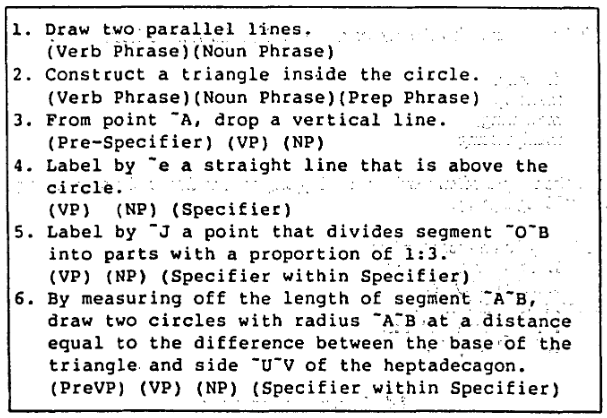
\includegraphics[width=10cm]{images/constructor_sentence_struct.png}
			\caption{Example of structured input sentences for CONSTRUCTOR.}
			\label{fig:constructorSentenceStruct}
		\end{figure}

	\item \textbf{Attribute Evaluation} - computes the basic features of grammatical structures, such as synthesized attributes.
		This computation will mostly involve synthesized attribute evaluation.

	\newpage
	\item \textbf{Semmantic Interpretation} - the semantic interpreter takes the results of all evaluations done before as input.
		The goal is to transform the English sentences into a \textit{metalevel} description intended for building complex noun phrases.
		\begin{figure}[h]
			\centering
			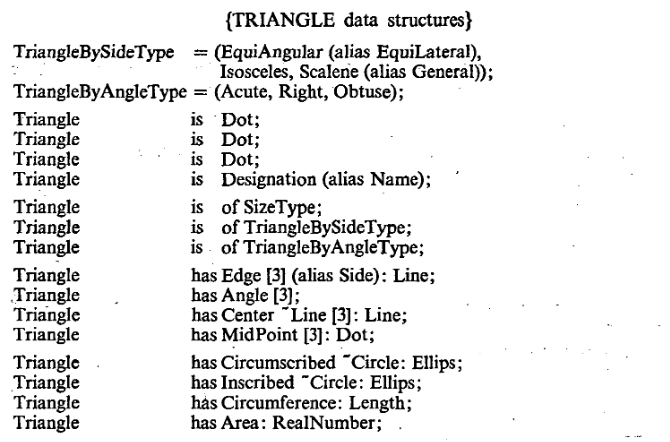
\includegraphics[width=12cm]{images/constructor_metalevel_desc.png}
			\caption{Example of a \textit{metalevel} description of CONSTRUCTOR.}
			\label{fig:constructorMetalevelDesc}
		\end{figure}
	
	\item \textbf{Construction Creator} - final component which takes a formal specification of an object, defining all the procedures to be executed.
		The results is a drawn geometric figure.
\end{itemize}

The purpose of exploring a tool of this type is not directly related to linguistics nor linguistic rules training.
The relevance of this reference is related to the use of attribute grammars with natural language processing, which techniques could be helpful when tacking a specific problem of this kind.


\section{VisualLISA (A Visual Programming Environment for Attribute Grammars)}
VisualLISA is a visual programming environment created by Nuno Oliveira in the year of 2009 \cite{oliveira_2009} for the specification of attribute grammars. 
Classified as a ``Domain Specific  Visual Language'', its main goal was to enhance the front-end of one other tool named LISA \footnote{https://labraj.feri.um.si/lisa/}, 
a compiler generator based in AG's that creates different visual tools based on the textual specification of the grammars.
    
The aim of this tool was to decrease the difficulty which is involved with specifying attribute grammars, not only for the LISA environment, but also regarding other types of systems, 
making specifications more visual and graphical.
    
Specifying grammars in a visual manner can be done using a set of icons (\autoref{fig:visuallisa_icons}) that must be combined to obtain the wanted result. 
Each icon or symbol has a unique function, and it is the users task to make the connections in a correct way.
    
% Imagem dos icons do VisualLISA
\begin{figure}[h]
    \centering
    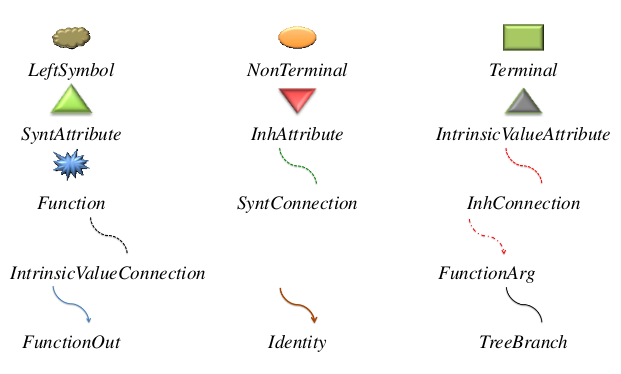
\includegraphics[width=10cm]{images/visuallisa_icons.png}
    \caption{VisualLISA set of icons.}
    \label{fig:visuallisa_icons}
\end{figure}

\newpage
The environment (\autoref{fig:visuallisa_window}) consists in 4 windows, each one with an individual task: 
declare the productions of the grammar in a textual manner; 
declare functions, data-types, etc.; 
draw the grammar productions; 
specify computation rules that were previously declared.
    
% Imagem da janela do VisualLISA
\begin{figure}[h]
    \centering
    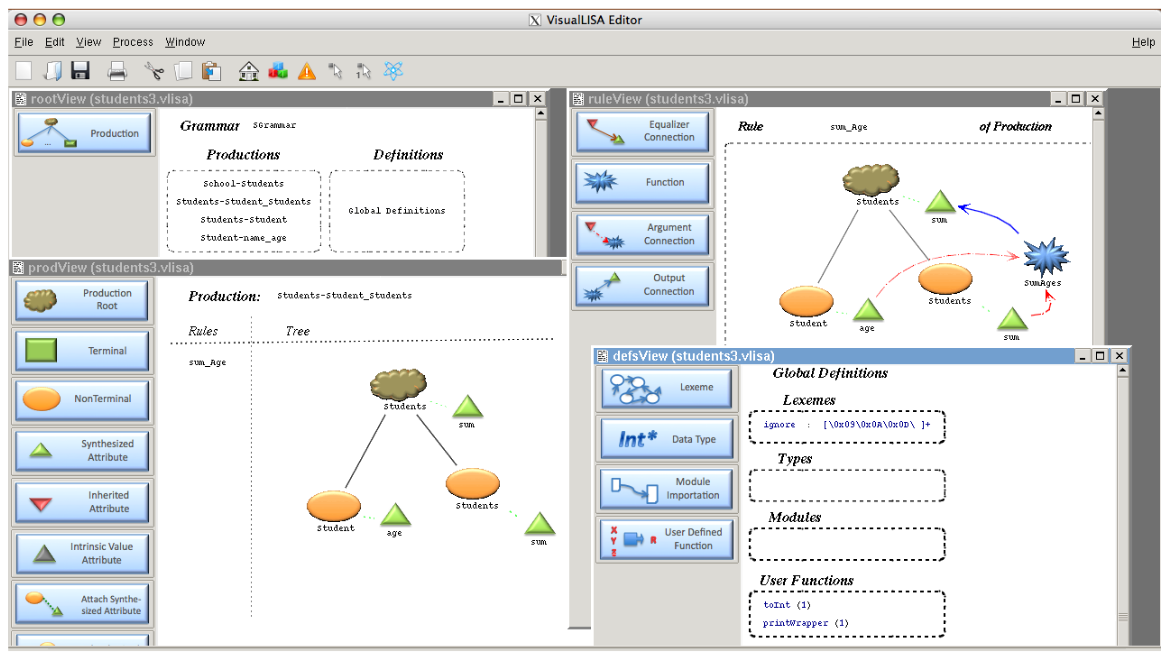
\includegraphics[width=10cm]{images/visuallisa_window.png}
    \caption{VisualLISA main window.}
    \label{fig:visuallisa_window}
\end{figure}
    
As an example, it was included a textual specification (\autoref{fig:textual_students_grammar}) 
and the respective graphical specification (\autoref{fig:graphical_students_grammar}), extracted from the paper \cite{oliveira_2009}.
    
% Students Grammar
\begin{figure}[h]
    \centering
    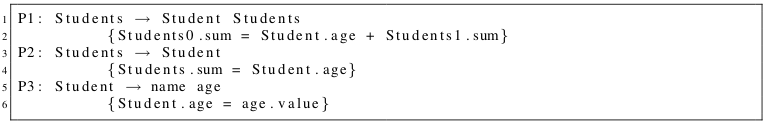
\includegraphics[width=15cm]{images/textual_students_grammar.png}
    \caption{Students textual grammar.}
    \label{fig:textual_students_grammar}
\end{figure}

\newpage

% VisualLISA Conception
\begin{figure}[h]
    \centering
    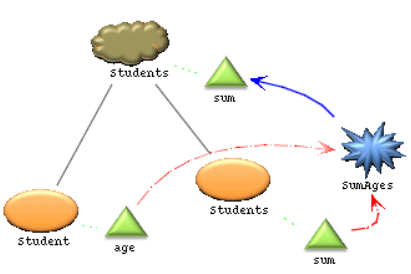
\includegraphics[width=8cm]{images/graphical_students_grammar.png}
    \caption{Students graphical grammar.}
    \label{fig:graphical_students_grammar}
\end{figure}

The main effect of the tool is not directly related to the problem that is trying to be solved, as the target users (linguists) may not be familiar with attribute grammars concepts such as 
terminal or non-terminal.
This can cause some confusion when working with all the icons provided by the platform in order to create the intended atttribute grammar.
Nevertheless, all the visual components that are associated could give some insights of interesting visual components to include/build when creating the proposed user interface to interact with the system.


\section{Chapter Summary} % TALVEZ ACRESCENTAR PEQUENA DESCRIÇÃO DE CADA SISTEMA????

In the previous sections, some tools were presented and major concepts discussed.
Some of the tools may not have a direct impact on the proposal of this thesis, but their research and inclusion on this document were crucial.
Each of the sections, despite their various differences, share the use of attribute grammars as a basis for a particular system,
or even to simplify their use thorugh various techniques.

The solution proposed is an approach that, despite using attribute grammars, 
it is based on a new textual \textsc{DSL} using \textsc{ANTLR} and the automated generation of processors in order to validate sentences.
In the next chapter, the proposal for this particular system will be discussed further.


% what is useful are all the visual components that are associated with it, 
% which could help when creating the intended user interface for the visual analysis of the generated 
% syntax-tree, or more. 
% Nevertheless, it is a very useful and interesting way of aproaching attribute grammars and their 
% specifications.

    
    %%%%%%%%%%%%%%% Chapter III - Architecture %%%%%%%%%%%%%%
    \chapter{Lyntax: Proposal}
    \label{cha:LyntaxProposal}
    \chapter{Lyntax: Proposal} \label{lyntax_proposal}

The main purpose of this proposal is the definition of a \textsc{DSL} that allows the specification of all different kinds of sentences, and afterwards, the possibility of testing given sentences as input and check if they are written accordingly to the rules previously specified. One obstacle that was encountered was how to extract the lexical part of the sentence, and in what way would each component be classified. In fact, this task is quite subjective, as different components may have various definitions in one context. % for example: (...). % Introduzir exemplo da professora!!!! 
Having known this, the decision was made that the student would beforehand identify the lexical part of the sentence.
% FALAR DO QUE VOU FAZER DE DIFERENTE (DICA DO LÁZARO!)


\section{System Architecture}
In order to specify all kinds of sentences/rules possible, the idea of creating a ``meta-language'' emerged. This ``meta-language'' will be used by the teacher to specify the rules for sentence construction. 
These rules will be written (in a single file) according to the following structure, that is divided into three main categories:

\begin{enumerate}
    \item \textbf{STRUCTURE} - the block where the teacher will write how is the sentence supposed to be written, and what components will it have.
    
    \item \textbf{ERRORS} - list of conditions that the teacher could write in order to be analysed afterwards, for example, certain values for different attributes. If one of the conditions is matched, an error will appear.
    
    \item \textbf{INPUT} - this block corresponds to the ``parsing'' of the sentence (the lexical part) that the student wants to test. This will be written by the student and then automatically joined with the teachers information.
\end{enumerate}

This file will then be processed by an \textsc{ANTLR} processor that will work on the information that was written, and then generate a grammar (also specified in \textsc{ANTLR}). This grammar corresponds to the translation of the
``meta-language'' into \textsc{ANTLR} instructions. Afterwards, the generated grammar will be used to create a validator of sentences, where the student can write his sentence/sentences and obtain results. 
These results would be the validation of the given sentence/sentences and a tree for a better visualization of the input structure.

% Imagem da arquitetura do sistema.
\begin{figure}[h]
    \centering
    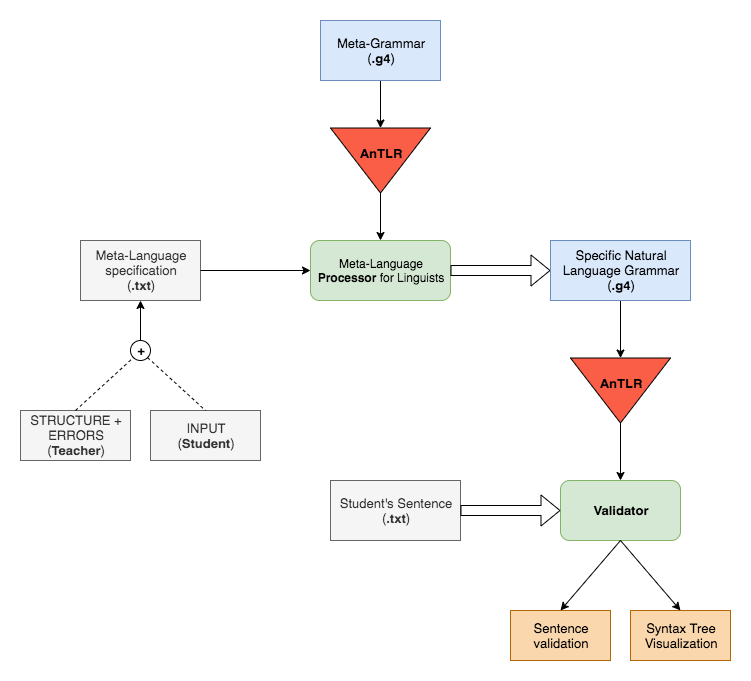
\includegraphics[width=10cm]{images/msc_system_architecture.png}
    \caption{System architecture.}
    \label{fig:system_architecture}
\end{figure}

\section{Meta-Language}
As it was stated in the beginning of this document, the main goal was to create a \textsc{DSL} that should be easy to learn and to rapidly understand and grasp. With this in mind, the structure mencioned before on the first section
of this chapter was followed: Three main parts, where two of them would be constructed by the teacher, and the third one was intended to be written by the student and later concatenated in a single file.

\subsection{Domain Specific Meta-Grammar}
The main intention of this language is to preprocess the information written by the teacher + student and then generate a validator for a particular structure. With simplicity in mind, a first version of the \textsc{DSL} was created, and it will be explained next.

\begin{center}
\begin{minipage}{8cm}
\begin{lstlisting}[language=java, basicstyle=\small, label={lst:processor_prod}, caption=Processor production]
processor : structure errors input
;
\end{lstlisting}
\end{minipage}
\end{center}

Firstly, the teacher specification will be discussed - meaning the \textbf{structure} and \textbf{errors} blocks.
The \textbf{structure} block is divided into \textbf{parts}, or main parts. These main parts correspond to the main components of the sentence. Each of these parts have an \textbf{element} within, containing the information about a certain component.

\begin{center}
\begin{minipage}{14cm}
\begin{lstlisting}[language=java, basicstyle=\small, label={lst:dsl_struct_prod}, caption=DSL structure/part/element productions]
structure : 'STRUCTURE:' (part)+ ;

part : 'part' '[' element ']' ;

element : '(' WORD ( '|' WORD )* ( ',' attributes )? ( ',' subparts )? ')' 
    ('?')? ;
\end{lstlisting}
\end{minipage}
\end{center}

The \textbf{element} is composed by the name of the component, a possible set of \textbf{attributes} and possible \textbf{subparts}.

\begin{center}
\begin{minipage}{13cm}
\begin{lstlisting}[language=java, basicstyle=\small, label={lst:dsl_attrs_prod}, caption=DSL attributes/subparts productions]
attributes : 'attributes' '{' WORD ( ',' WORD )* '}'
;

subparts : 'subparts' '[' element ( ',' element ) ']'
;
\end{lstlisting}
\end{minipage}
\end{center}

The \textbf{subparts} production intends to be the path for ``injecting'' more elements inside a single component. One component may be composed by several other components. As shown in the example above, the \textbf{subparts} production is a list of one or more elements.

Secondly, the teacher can define a list of restrictions to be applied to each attribute defined in the previous structure. A sentence will be valid if it follows the specified structure and if it obeys to the specified conditions.

\begin{center}
\begin{minipage}{12cm}
\begin{lstlisting}[language=java, basicstyle=\small, label={lst:dsl_errors_prod}, caption=DSL errors/expression productions]
errors : ('RULES'|'ERRORS') ':' ( condition ';' )+
;

condition : assignment ( ('AND'|'OR') assignment )*
;
\end{lstlisting}
\end{minipage}
\end{center}

The \textbf{errors} production will have two meanings: if the keyword use is 'RULES', then the conditions defined by the teacher need to be checked in order for a sentence to be correct; on the other hand, if the keyword is 'ERRORS', then if the conditions are matched, the sentence is not considered correct within that structure.
The \textbf{condition} production is composed by a set of assignments that can be joined using the logical operators 'AND' and 'OR'. 
Each condition intends to create logical evaluations for the various attributes defined.
Conditions are composed by assignments, which are composed by expressions.

\begin{center}
\begin{minipage}{10cm}
\begin{lstlisting}[language=java, basicstyle=\small, label={lst:dsl_cond_prod}, caption=DSL condition production]
assignment 
    : expression ('='|'!=') expression
    | expression ('='!'!=') '"' WORD '"'
;

expression : WORD ( '.' WORD )* '->' WORD 
;
\end{lstlisting}
\end{minipage}
\end{center}

The \textbf{assignment} production assigns an \textbf{expression}, which is composed by the path to a certain attribute, to a value or to other expression. 
If, for instance, the teacher says that an attribute is equal to some value, then the student can not use other value to that attribute - this would result in an error.

Thirdly, and finally, the \textbf{input} block, which corresponds to the students section. This was treated has a different and separate \textsc{DSL}, as its main purpose was to identify the lexical parts of the sentence written 
by the student, allowing for a correct and non-subjective parsing of each word in the sentence.

\begin{center}
\begin{minipage}{8cm}
\begin{lstlisting}[language=java, basicstyle=\small, label={lst:dsl_input_prod}, caption=DSL input production]
input : 'INPUT:' phrase 
;

phrase : ( '-' parts )+
;
\end{lstlisting}
\end{minipage}
\end{center}

The sketch starts within a section named \textbf{phrase}, which corresponds to one sentence in particular. 
This production is composed by one or more \textbf{parts}, each of them holding various \textbf{blocks}, where all the information is stored. 
Inside, the name of the components and their required attributes must be specified. 
It is also important to notice that a correct path must be specified by the student. 
If the student specifies a component that is not declared in the structure defined previously by the teacher, then an error should be thrown.

\begin{center}
\begin{minipage}{10cm}
\begin{lstlisting}[language=java, basicstyle=\small, label={lst:dsl_parts_prod}, caption=DSL parts/component/content productions]
parts : '(' block ( ',' block )* ')'
;

block : WORD content
;

content : (slice)? (attrs)? (parts)?
;
\end{lstlisting}
\end{minipage}
\end{center}

The student can specify the \textbf{slice} of the sentence that corresponds to the component that is being declared, and a set of attributes (\textbf{attrs}) that composes said component. Furthermore, it is possible to continue to define more \textbf{parts} within one part, just like the teacher's \textsc{DSL} \textbf{subparts}.

\begin{center}
\begin{minipage}{11cm}
\begin{lstlisting}[language=java, basicstyle=\small, label={lst:dsl_slice_prod}, caption=DSL slice/attrs/evaluations/eval productions]
slice : ':' '``' (WORD)+ '"'
;

attrs : '[' evaluations ']'
;

evaluations : eval ( ',' eval )*
;

eval : WORD '=' '``' WORD '"'
;
\end{lstlisting}
\end{minipage}
\end{center}

Inside the \textbf{slice} production, a list of words can be written. These are the words that will then be used to build the lexical part of the generated grammar. Also, when specifying attributes, the student must assign a value for each attribute that will then be used to validate each component of the sentence.

For a better understanding of the three main categories (structure, errors and input), bellow there is an example that is based on the first case study, and shows what the specification of the teacher should look like.

\begin{center}
\begin{minipage}{13cm}
\begin{lstlisting}[language=java, basicstyle=\tiny, label={lst:metaStruct}, caption=Example of a possible sentence structure]
STRUCTURE:
	part[(
        Sujeito, 
        attributes{tipo}, 
        subparts[
            (Determinante)?, 
            (Nome)
        ]
	)]
    
	part[(
        Predicado,
        subparts[
            (Verbo, attributes{tipo}),
            (Complemento_Direto, subparts[(Determinante)?, (Nome)]),
        ]
	)]

ERRORS:
    Sujeito->tipo = ``animado" AND Predicado.Verbo->tipo = ``inanimado";
    Sujeito->tipo = ``inanimado" AND Predicado.Verbo->tipo = ``animado";
\end{lstlisting}
\end{minipage}
\end{center}

In the case of the student, this is the specification that should be used and one of the many examples that fit into the defined structured.

\begin{center}
\begin{minipage}{13cm}
\begin{lstlisting}[language=java, basicstyle=\tiny, label={lst:metaInput}, caption=Example of the students parsing]
INPUT:
    - (Sujeito: ``O Carlos" [tipo = ``animado"]
        (Determinante: ``O", Nome: ``Carlos"))
    - (Predicado: ``teme a sinceridade" 
        (Verbo: ``teme" [tipo = ``animado"], Complemento_Direto: ``a sinceridade" 
            (Determinante: ``a", Nome: ``sinceridade")))
\end{lstlisting}
\end{minipage}
\end{center}


\section{Chapter Summary}

In this chapter, it was discussed the different phases of the proposes system architecture and what the output of a system like this should be.
The principle is to create a new Domain Specific (Meta) Language that allows for the specification of sentence structures as well as proper input.
Within this system, a processor for this Meta-Language is created by using \textsc{ANTLR},
which evaluates the specification written and is tasked with the generation of a specific natural language grammar.
Combining the newly generated grammar with \textsc{ANTLR}, the result is a student's sentence validator
that when given a sentence as input, performs all the necessary validations and, if correct, presents the user the respective syntax tree.

\textbf{Lyntax}, the word that combines the terms ``Linguistics" and ``Syntax", was the name chosen for a system that combines both the meta-language processor and
the user interface that makes use of such processor. The process of the implementation of this system will be discussed next.


    %%%%%%%%%%%%%%%%% Chapter IV - Prototype %%%%%%%%%%%%%%%%
    \chapter{Lyntax: Development}
    \label{cha:LyntaxDevelopment}
    \chapter{Lyntax: Development} \label{lyntax_development}

This chapter will present the development and workflow of the system. 
As previously mentioned, the next step was to expand the defined DSL, and to use attributes as a form of calculation. 
Most of the productions were expanded, allowing for certain calculations to be injected over the tree.


\section{Meta-Grammar}

With the grammar divided into 3 main parts (STRUCTURE, ERRORS, INPUT), different types of calculations occur at different sections. The STRUCTURE and ERRORS blocks are written in a single file (by the teacher) which is then joined 
with the INPUT block (written by the student). The process starts with searching for the teacher and student specification, and then compiling the program using a meta-grammar based processor. A new processor is generated to be 
used by the student to verify if his sentences are correctly following the structure defined by the teacher. Within the grammar itself, the first rule, 

%\begin{center}
%\begin{minipage}{11cm}
%\begin{Verbatim}[frame=single, framesep=2mm, fontsize=\small]
%determinante returns[Integer genero, Integer numero]
%    : ('A' | 'a')
%        { $genero = FEMININO; $numero = SINGULAR; }
%    | ('O' | 'o')
%        { $genero = MASCULINO; $numero = SINGULAR; }
%    | ('As' | 'as')
%        { $genero = FEMININO; $numero = PLURAL; }
%    | ('Os' | 'os')
%        { $genero = MASCULINO; $numero = PLURAL; }
%
%    (...)
%;
%\end{Verbatim}
%\end{minipage}
%\end{center}

\begin{center}
\begin{minipage}{11cm}
\begin{lstlisting}[language=java, basicstyle=\small, label={lst:processor}, caption=Processor rule from the meta-grammar]
processor
@init {
    /* Main data structure. */
    List<RoseTree> struct = new ArrayList<>();

    (...)
}
    : structure[struct]
      errors[struct]
      input[struct]
    {
        (...)
    }
\end{lstlisting}
\end{minipage}
\end{center}

\noindent starts by initializing the main data structure. This structure is responsible for storing all the information that is being parsed from the file given as input (the meta-language file). 

When choosing the correct structure to store all the important data, the first \/\*approach\*\/ taken was to store all components in a single Map, with each name of a component
matching their respective value. The problem with this approach, which was identified right away, was that is possible to exist two or more components with the same exact
name, causing a conflict within the Map. Furthermore, components have different information associated, like attributes, and it would be better if it is all in the same
place - this created the need for a Component class.

The Component class would store the name of the component, a possible value and a Map that associated each attribute with some value. The components would all be stored
within a List.
\newpage

\begin{center}
\begin{minipage}{10cm}
\begin{lstlisting}[language=java, basicstyle=\small, label={lst:component_class}, caption=Component class]
@members {
    class Component {
        String name;
        String lexical_part;
        Map<String, String> attributes;
    }

    /* Main data structure. */
    List<Component> struct;
}
\end{lstlisting}
\end{minipage}
\end{center}

The problem with this solution is that it does not follow any particular order (in this case, the STRUCTURE order), which can be very useful when validating the students.
The sequence of components stored within a List would not be equal to the sequence of components that were defined in the structure previously defined.

The structure of the sentence takes a form of a tree, so that would be the correct way to store the information and maintain order. As each node could have less or more 
than two children, a binary tree was not the way to go. The idea was to build a Graph structure that used a mapped each node to a list of nodes.

\begin{center}
\begin{minipage}{11cm}
\begin{lstlisting}[language=java, basicstyle=\small, label={lst:graph_class}, caption=Graph class]
@members {
    class Graph
    {
        Map<Component, List<Component>> map;
    }
}
\end{lstlisting}
\end{minipage}
\end{center}

Although this could maintaing the order, the initial problem remainded. We could have components with the same exact properties, and this would cause conflict between
edges, and not create a new node when it was supposed to.

The principle of having a tree as the main data structure falls into the need of maintaining a valid path. For example, if the teacher says that the structure will have a component \emph{\textbf{A}}, and this component has two children, \emph{\textbf{B}} and \emph{\textbf{C}}, then the paths \emph{\textbf{A$\rightarrow$B}} and \emph{\textbf{A$\rightarrow$C}} should be stored. In this particular problem, it is required to have a tree that within each node has a list of children with an arbitrary size of \emph{\textbf{N}}.

Some backtracking was made to come up with an ideal solution. The prerequisites were that order needed to be maintained and each node (component) had an arbitrary number
of \emph{\textbf{N}} children. The previously created Component class would store all its values and a list of new components (children), creating a path between 
the parent component and said children. This type of structure is denominated as Rose Tree, which is a prevelant structure within the functional programming community. 
It is a multi-way tree, with an unbounded number of branches per node. This way, all the prerequisites would be matched, and all the information correctly stored. 

\begin{center}
\begin{minipage}{10cm}
\begin{lstlisting}[language=java, basicstyle=\small, label={lst:rosetree_class}, caption=RoseTree class]
class RoseTree {
    String chosenValue;
    String path;
    boolean visited;
    boolean required;
    Map<String, String> attributes;
    Set<String> optionValues;
    List<String> lexical_part;
    List<RoseTree> children;

    (...)
}
\end{lstlisting}
\end{minipage}
\end{center}

When in the main production (\emph{processor}), a list of \emph{Rose Trees} is initialized, with each tree of the list corresponding to the main components of the sentence. This structure would travel along the parsing tree, to first be populated with information and then serving as the main source of validation and checking.

On the first block (STRUCTURE) there are not many calculations happening within the productions. 
The main task is to simply validate the syntax and extract data to be stored in the \emph{Rose Tree}. 
For each node, it is stored the name of the component, if it is required to be declared or not, a group of attributes (could be non-existent), 
a lexical part (if it is the case), and finally a list of nodes, referred as the children.

After the parsing of the structure, there are a list of conditions named ERRORS that need to be validated and converted into \emph{Java} syntax - this conversion would then be injected on the main rule of the generated grammar. These logical expressions are based on the attributes of each component and their relations. For example, if the teacher says that a component \emph{\textbf{A}} has an attribute named \emph{\textbf{a}}, and this attribute is required to have value \emph{\textbf{x}}, if the student assigns it a value of \emph{\textbf{z}}, then an error should appear. All these conditions can be combined with the logical operands ``AND'' or ``OR''. The way that is parsed is based on the path specified by the teacher when accessing the attribute. Using the example before, a component \emph{\textbf{A}} with a child \emph{\textbf{B}}, with \emph{\textbf{B}} having a attribute \emph{\textbf{x}}, in order to access it, the syntax should be

\[ A.B -\textgreater x \]

\noindent as the full path is required. This is done in order to calculate the correct path and avoid ambiguity between attributes. Over the parsing of these rules, the path is being validated, and in case of any error, the user is notified.

Finally, the last block corresponds to the input that was written by the student. 
The goal is to validate the components that were defined, and match them with the structure created by the teacher. 
Again, the RoseTree was used as a way to check if the student’s components and paths were valid. 
The task of the student was to ``parse'' his sentence and divide it by components, identifying the lexical segments and storing them within a node of the \emph{Rose Tree}. 
At last, the main rule of the Meta-Grammar makes use of a generator to generate all the rules for the Specific Natural Language Grammar. 
Within this generator, the various \emph{Rose Tree's} are passed as an argument and then traversed recursively.
% In the case of any error, the user is informed of where the error happened but also in which component. 
% Furthermore, when parsing attributes and their respective values, if the student defines two attributes with the same name, but with different values, 
% a warning is raised to inform the user that the value that was considered was the last one to be recognized.


\section{Meta-Language Processor}

In order to simplify the usage of the Meta-Grammar, and as the grammar itself made use of auxiliar \emph{Java} classes, all of that was combined into a \emph{JAR} file.
Having this type of package would allow for a more flexible integration with any component.
The Meta-Language Processor, which was created by providing the Meta-Grammar file to ANTLR, could now be used with the \emph{JAR} file, 
providing as input the Meta-Language Specification. 

\begin{figure}[h]
    \centering
    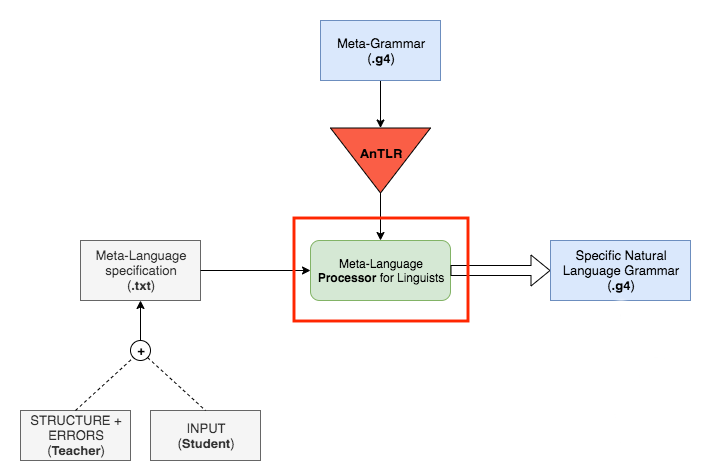
\includegraphics[width=9cm]{images/system_meta_processor.png}
    \caption{Excerpt of the system architecture - Meta Processor.}
    \label{fig:system_architecture}
\end{figure}

\newpage
\noindent Using the command line, the instruction:
\begin{Verbatim}
	java -jar lib/MetaGrammar.jar input/meta-lang
\end{Verbatim}
\noindent tries to generate the Specific Natural Language Grammar, based on the input provided. In case of any error, the grammar would not be generated.


\section{Specific Sentence Grammar Generator}

As previously mencioned, the role of this generator is to produce the grammar that intends to recognize the students input.
This grammar is specific to the sentence, and contains the conditions previously defined by the teacher ready to be evaluated.
The generator is an auxiliar \emph{Java} class, which contains the methods necessary to traverse the RoseTree given as argument,
and create the strings of text for the grammar, which will then be appended to a file.

The principle of this generator is to create the independent strings first, and then recursively traverse the tree in order to create the productions themselves.
This task was done using an auxiliar data structure,
\begin{Verbatim}
	Map<String, StringBuilder> productions 
		= LinkedHashMap<>();
\end{Verbatim}
\noindent with each \underline{key} representing the name of a production, and each \underline{value} representing the various words that composed the rule of said production.
The chosen structure would be a \emph{Linked Hash Map}, as the insertion order was important to maintain.
While traversing the tree, the information would be processed and also stored within the auxiliar Map.
Lastly, all strings containing the productions, and also a lexer, are printed into a file of type ``.g4". 
This is the file containing the grammar which will then be use to create the sentence validator.

\newpage
\section{Sentence Validator}

If no errors occur in the previous step, we should now have a file named ``Grammar.g4" that corresponds to the Specific Natural Language Grammar.
This grammar contains all the tokens extracted from the Meta-Language specification, and combining it with ANTLR, we create a new specific Sentence Validator.
When providing the student's sentence to the Sentence Validator, and if all goes well, a Syntax Tree should be generated using a tool called \emph{TestRig}.
Using the command line once again, and providing a specific flag to the tool (\emph{-gui}), we obtain the final syntax tree for the sentence provided: 
\begin{Verbatim}
	java -cp \ 
		"lib/antlr-4.8-complete.jar:$CLASSPATH" \ 
		org.antlr.v4.gui.TestRig \ 
			Grammar main input/sentence \ 
		-gui
\end{Verbatim}

\begin{figure}[h]
    \centering
    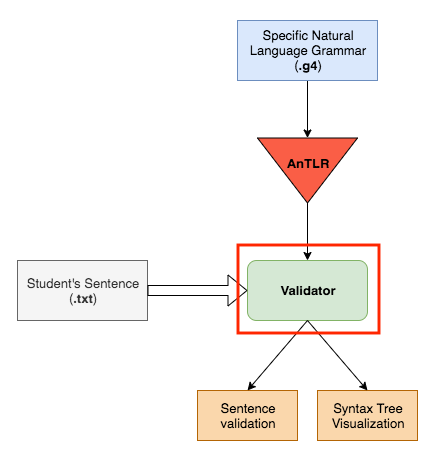
\includegraphics[width=7cm]{images/system_sentence_validator.png}
    \caption{Excerpt of the system architecture - Sentence Validator.}
    \label{fig:systemSentenceValidator}
\end{figure}

\noindent As an example, using \autoref{lst:metaStruct} and \autoref{lst:metaInput}, the generated syntax tree would be:
\begin{figure}[h]
    \centering
    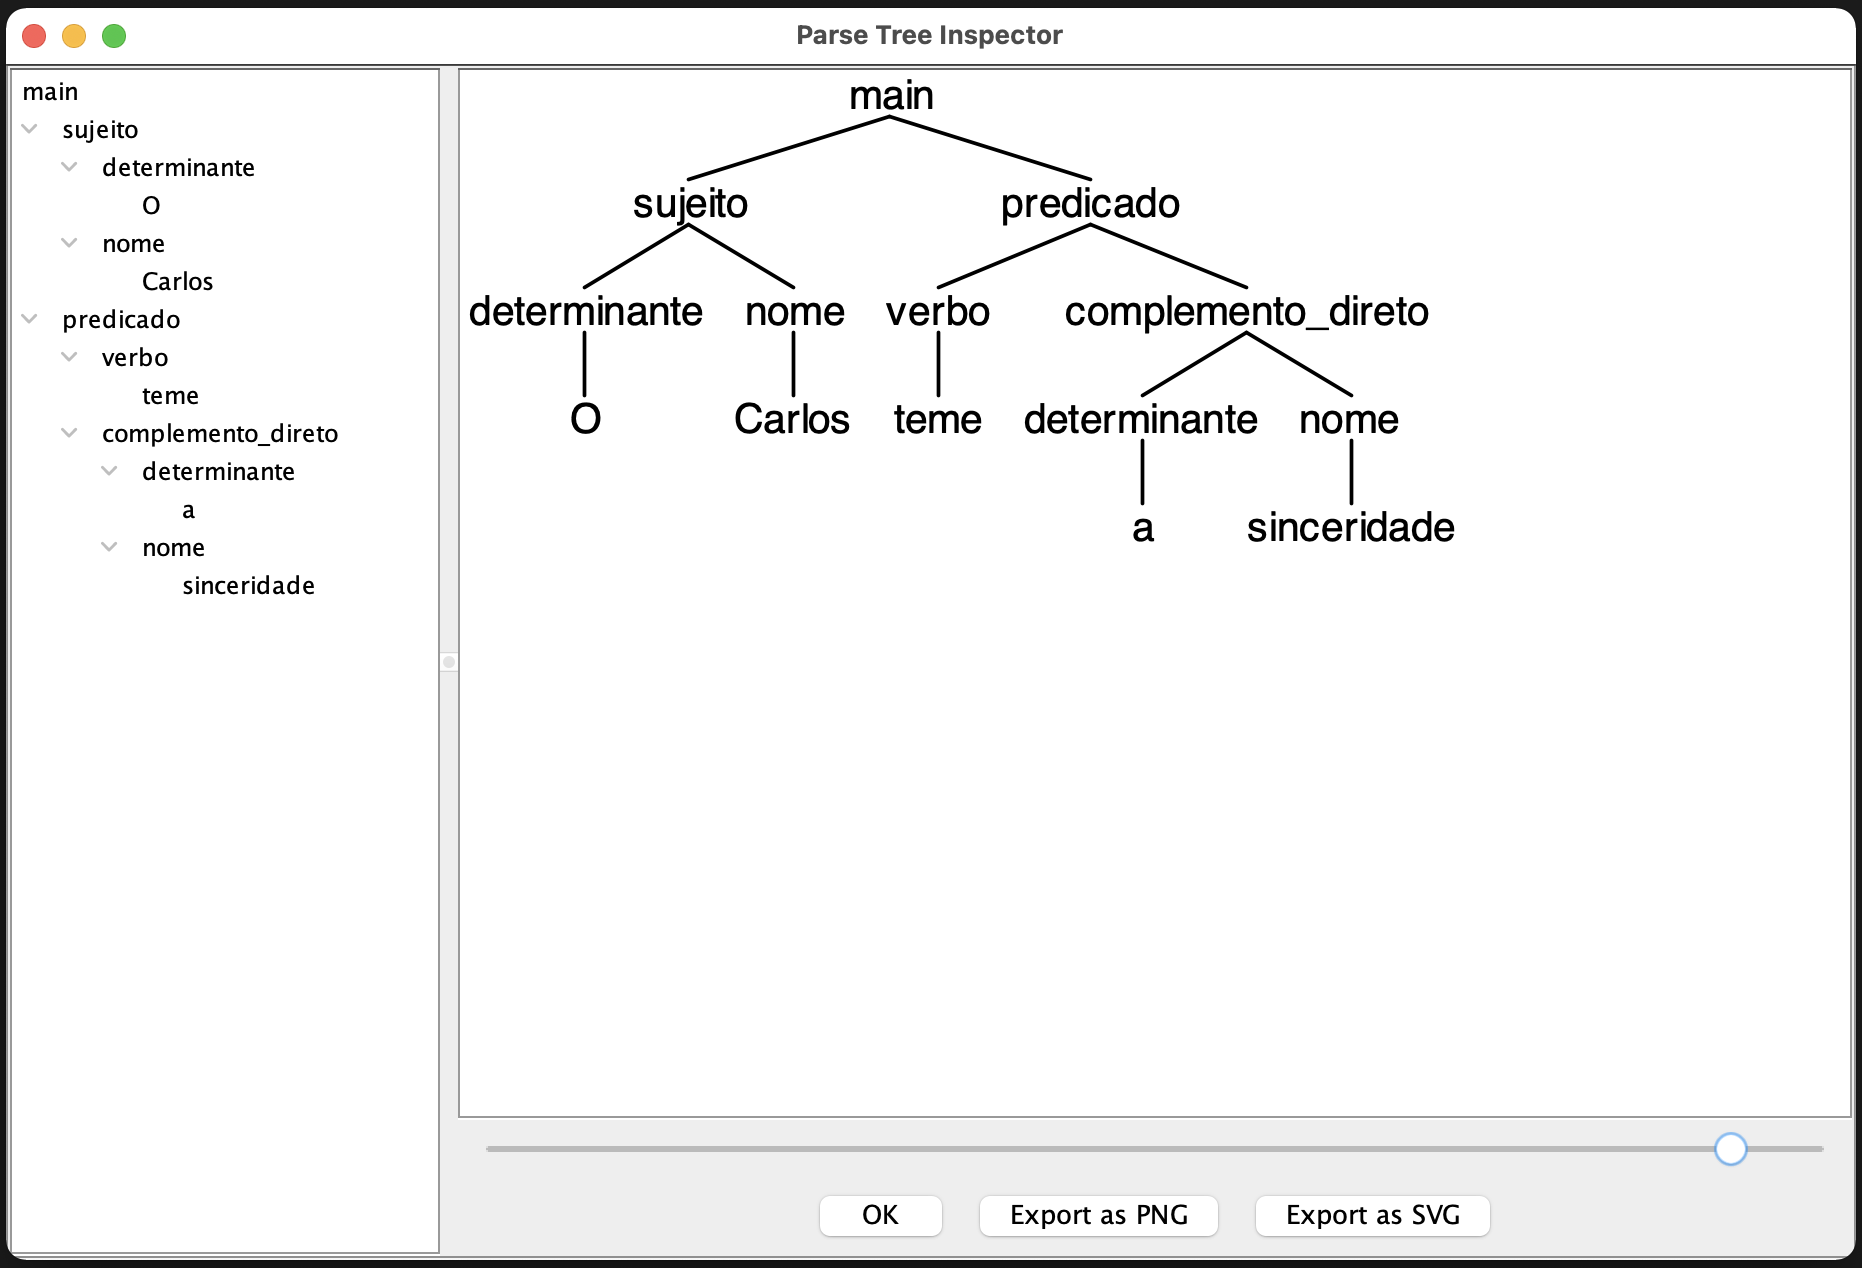
\includegraphics[width=11cm]{images/testrig_gui_example.png}
    \caption{Example of a generated syntax tree within TestRig.}
    \label{fig:testrigGuiExample}
\end{figure}

\newpage
\section{Lyntax: Interface}

As stated in the introduction of this document, after the creation of a system capable of testing various sentences, the goal was to build an user interface
that allowed for a more easy and simple use of said system, without the need of directly using the command line for providing inputs or manual runtime compilations.
The interface was built using \emph{\textbf{Swing}}, a GUI widget toolkit for \emph{Java}.
\emph{Swing} has a lot of sophisticated GUI components available for use, allowing the developer to focus on pure functionality.
Furthermore, using the \emph{NetBeans} \footnote{https://netbeans.org/} IDE (Integrated Development Environment) for \emph{Java}, it was possible to use a GUI builder for manipulating \emph{Swing} components, 
by dragging and dropping them to a canvas - this would generate the specific \emph{Java} code for each component.

Objectively, the front-end part of the system would consist on a single window composed by two main text areas, corresponding to the rules and input blocks,
one button to generate the specific sentence validator and one last button to inject the sentence into the validator and giving the user their sentence syntax tree.
The window would also have a top menu bar that would allow the user of opening text files if desired.
In any case, the user could write the STRUCTURE, ERRORS/RULES and INPUT blocks directly into the respective text areas without opening any file. 

\begin{figure}[h]
    \centering
    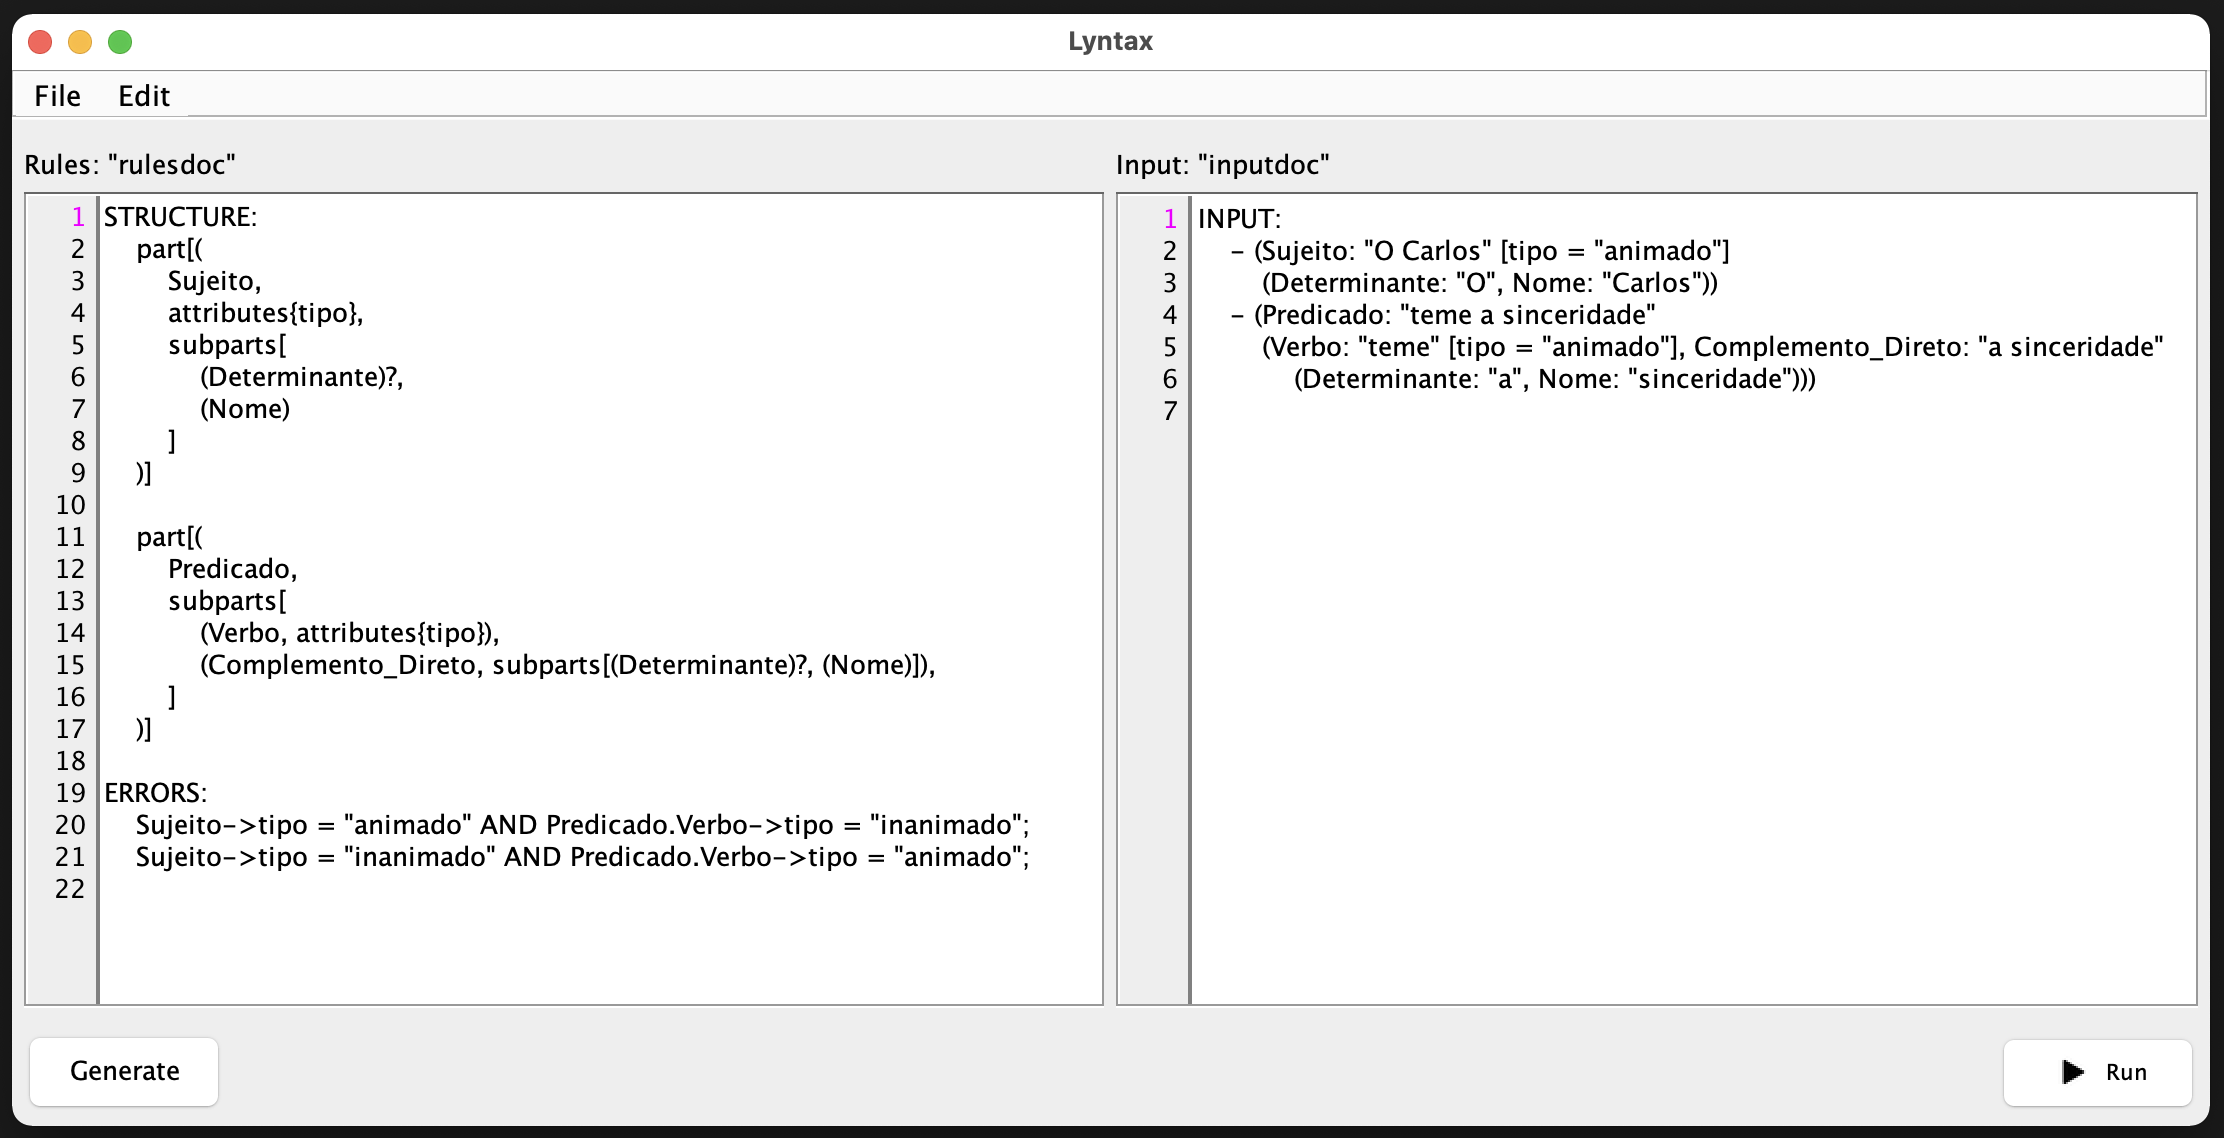
\includegraphics[width=14cm]{images/lyntax-gui.png}
    \caption{Lyntax user interface.}
    \label{fig:lyntaxGui}
\end{figure}

After the specification of the rules (in the left side) and input (in the right side), the user can generate the Specific Natural Language Grammar to be able to create the Sentence Validator,
using the ``Generator" button.
The text within the two text boxes is concatenated, and given as input for the MetaGrammar processor.
All these operations are done in background, following the same order as the instructions showed above.
If all goes well, the user should have prompted a message saying that the Grammar was successfully generated - it is now possible to test the sentence.

\begin{figure}[h]
    \centering
    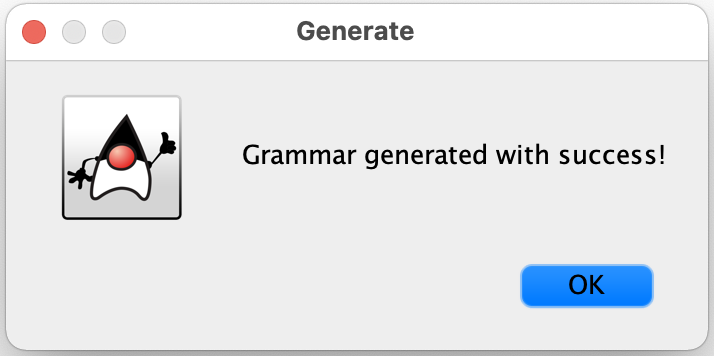
\includegraphics[width=5cm]{images/grammar_gen_success.png}
    \caption{Grammar generation success message.}
    \label{fig:grammarGenSuccess}
\end{figure}

\newpage
At last, by clicking the ``Run" button, the validator is created, and the sentence passed as input.
If no errors occur during this process, the user should see the sentence syntax tree as the one used in \autoref{fig:testrigGuiExample}.
On the other hand, if errors or warnings occur, they are displayed textually for the user in a small window.

\begin{figure}[h]
    \centering
    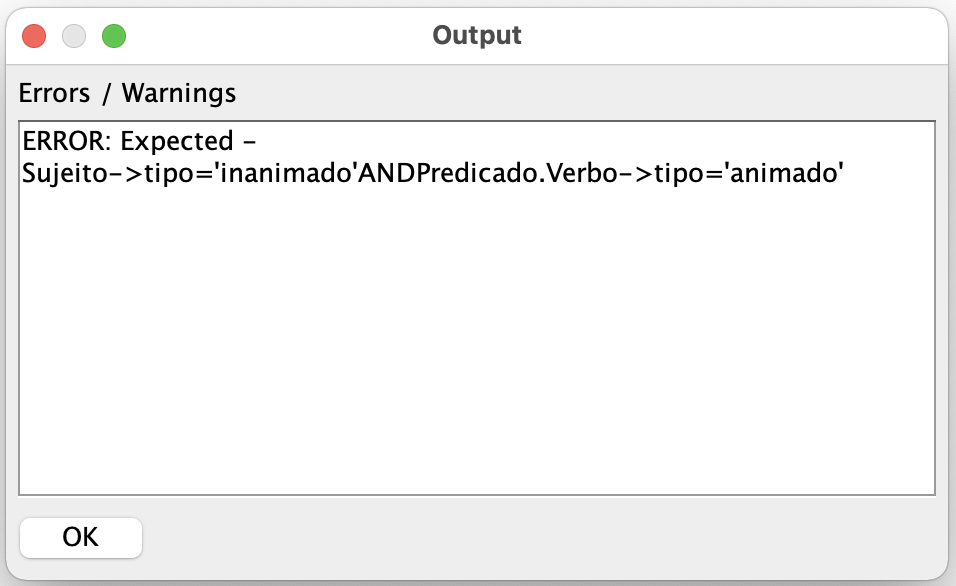
\includegraphics[width=7cm]{images/lyntax_error_window.png}
    \caption{Example of an error message.}
    \label{fig:lyntaxErrorWindow}
\end{figure}


\section{Lyntax: Website}

...

\section{Chapter Summary}

At this stage, the development of the system is concluded.
The result was, firstly, a DSL that allows for the specification of sentence structures and rules, as well as a respective input for those same structures.
Secondly, the core system which processed the Meta-Language specification, generated a specific grammar, 
and then used that grammar to create a validator for the analysis and evaluation of a specified sentence.
At last, and as a way of abstracting the complexity of the core system, 
the front-end intends to deliver a more flexible and straight forward use of the tool,
allowing the user to focus on the description of the rules and testing of sentences.

The main challenges faced over the development period were, firstly,
to choose the most appropriate data structure which would then be used to manipulate and process input data.
As previously discussed, this structure demanded for a set of specified requirements to be met in order to produce correct results, 
so this task took quite a few tries and experiments to get right and accurate.
Lastly, the error handling of the tool may cause some confusion at first, as it is handled and processed within the Meta-Grammar processor.
This error message is then passed onto the specific natural language grammar, and printed to the user into a formatted window to ease the process.
Nevertheless, the rules errors are precise and easy to understand.

Within the next chapter, some case studies will be explored in order to prove the correct functioning of the system.

% Having parsed the meta-language file, a generator is called by the main rule - the \emph{Rose Tree} is passed as an argument and then traversed in order to generate all 
% the rules for the Specific Natural Language Grammar.
% This grammar, after being generated, is used to create a processor in which the student's sentence will be used as input, creating a visual 
% syntax tree of that same sentence.

    
    %%%%%%%%%% Chapter V - Experimental Evaluation %%%%%%%%%%
    \chapter{Case Studies}
    \label{cha:CaseStudies}
    \chapter{Case Studies} \label{case_study}
In order to better explain the solution architecture presented in this thesis, some concrete examples will be presented in this section. 
The main idea is to show the specifications used by the teacher and by the student and how the generator processor verifies the correcteness of the student sentences. 
The DSL design consists in slicing the sentence into parts, and each part can have subparts.

\textbf{Lyntax}, the word that combines the terms ``Linguistics" and ``Syntax", was the name chosen for a system that combines both the meta-language processor and
the user interface that makes use of such processor.
These case studies are also relevant as an example for a possible pedagogical scenario by using the system in a classroom context.
The purpose of this chapter is to also demonstrate some of the process in which both the Teacher and Student will be involved, and to exhibit some common structures
and inputs as well as their results.

\section{Attribute Validation}
This case study intends to demonstrate the validation on sentence components based on their attributes. The example showed in the previous chapter 
\autoref{lst:metaStruct} contains a structure that is composed by two main parts: a subject (\underline{Sujeito}) and a predicate (\underline{Predicado}). 
The subject is then subdivided into a possible determiner (\underline{Determinante}) and a noun (\underline{Nome}), which are then matched with a word 
(the lexical part identified by the student). The predicate is composed by a verb and a complement that is directly related to the verb. This complement 
(\underline{Complemento\_Direto}) is then composed by a possible determiner (\underline{Determinante}) and a mandatory noun (\underline{Nome}).

In this particular example, both the subject and the verb from the predicate have an attribute named ‘tipo’ which purpose is to check evaluate if each of the components
are animated or inanimated. By analysing the logic in the ERRORS block \autoref{lst:metaStruct}, we can see that if the value of the attribute ‘tipo’ is different 
between the two components, than an error should be pointed. In this case, the sentence parsed by the student is

``O Carlos teme a sinceridade.''

\noindent which is in fact a valid sentence, as the name ``Carlos'' and the verb ``teme'' are both animated.

When running the example above (\autoref{lst:metaStruct} plus \autoref{lst:metaInput}) in the Meta Grammar processor, and if no errors occur, a specific grammar (in ANTLR) 
in then generated. For this specific case, this is the generated grammar.

\begin{center}
\begin{minipage}{15cm}
\begin{lstlisting}[language=java, basicstyle=\tiny, label={lst:case_study_sentence}, caption=Example of a specific generated grammar.]
grammar Grammar;

@members {
    final String Sujeito__TIPO = ``animado";
    final String Predicado__Verbo__TIPO = ``animado";
}


main : sujeito predicado
{
    if ( Sujeito__TIPO.equals(``animado") && Predicado__Verbo__TIPO.equals(``inanimado") ) 
        { System.out.println(``ERROR!"); }

    if ( Sujeito__TIPO.equals(``inanimado") && Predicado__Verbo__TIPO.equals(``animado") ) 
        { System.out.println(``ERROR!"); }
}
;

sujeito : (determinante)? nome 
;

determinante : 'O' | 'a'
;

nome : 'Carlos' | 'sinceridade'
;

predicado : verbo complemento_direto 
;

complemento_direto : (determinante)? nome 
;

verbo : 'teme'
;


/* LEXER */
(...)
\end{lstlisting}
\end{minipage}
\end{center}

In the ‘main’ production, we can see the logical conditions that are ready to be evaluated when running this grammar. As the conditions are false, no errors should occur,
allowing for the visualization of the syntax tree.

% INSERIR PRINT DO TESTRIG????

%To conclude, if we use as an input a sentence like
%
%``O Carlos teme a sinceridade.''
%
%\noindent the sentence is accepted because, firstly, the structure is correct, and every component is in the right place, and secondly, all the attributes obey to the rules. As another example, if we use as an input other sentence for example
%
%``O acidente teme a sinceridade.''
%
%\noindent we get an error which indicates that the verb ``teme'' requires an animated subject, and ``acidente'' belongs to the subject that has an inanimated property.
%
%\begin{center}
%\begin{minipage}{10cm}
%\begin{lstlisting}[language=java, basicstyle=\small, label={lst:error_message_dsl}, caption=Example of an error message]
%ERRO:
%- O verbo 'teme' requer um sujeito ANIMADO.
%\end{lstlisting}
%\end{minipage}
%\end{center}

\section{Missing components \& Warnings}
Still based on the previous defined structure \autoref{lst:metaStruct}, the student's specification can still be missing some components that are mandatory. 
This case study just intends to show the way that errors or warnings are notified to the user.

In order to demonstrate this, the input block defined above \autoref{lst:metaInput} is going to suffer some modifications in order to trigger errors or warnings.

\begin{center}
\begin{minipage}{13cm}
\begin{lstlisting}[language=java, basicstyle=\small, label={lst:meta_input_missing_comp}, caption=Example of the students parsing with missing component]
INPUT:
    - (Sujeito: ``O Carlos" [tipo = ``animado"]
        (Determinante: ``O"))
    - (Predicado: ``teme a sinceridade" 
        (Verbo: ``teme" [tipo = ``animado"], 
         Complemento_Direto: ``a sinceridade" 
            (Determinante: ``a", Nome: ``sinceridade")))
\end{lstlisting}
\end{minipage}
\end{center}

In this example, we can see that within the subject component (\underline{Sujeito}), the noun component (\underline{Nome}) is not defined. 
This particular case would cause an error as the noun component is mandatory (based on the previous structure \autoref{lst:metaStruct}). 
The error message identifies the missing component.

\begin{center}
\begin{minipage}{13cm}
\begin{lstlisting}[language=java, basicstyle=\small, label={lst:err_msg_missing_comp}, caption=Example error message of missing component]
ERROR: (INPUT) 
- The mandatory component 'Nome' has not been defined.
\end{lstlisting}
\end{minipage}
\end{center}
Another possible error would be to not define attributes, and to not give those attributes values. In this case, if we remove the attribute ‘tipo’ from the subject 
component (\underline{Sujeito}),

\begin{center}
\begin{minipage}{13cm}
\begin{lstlisting}[language=java, basicstyle=\small, label={lst:meta_input_missing_attr}, caption=Example of the students parsing with missing attribute]
INPUT:
    - (Sujeito: ``O Carlos"
        (Determinante: ``O", Nome: ``Carlos"))
    - (Predicado: ``teme a sinceridade" 
        (Verbo: ``teme" [tipo = ``animado"], 
         Complemento_Direto: ``a sinceridade" 
            (Determinante: ``a", Nome: ``sinceridade")))
\end{lstlisting}
\end{minipage}
\end{center}

\noindent the error should notify the user that the subject component is missing attributes, as attributes are always mandatory (if the component related to them is also
mandatory).

\begin{center}
\begin{minipage}{14cm}
\begin{lstlisting}[language=java, basicstyle=\small, label={lst:err_msg_missing_attr}, caption=Example error message of missing attributes]
ERROR: (INPUT)
- There are attributes related to the component 'Sujeito' that were not defined.
\end{lstlisting}
\end{minipage}
\end{center}

When it comes to warnings, there is only one case that raises them. This happens when the user defines the same attribute multiple times, warning that only the last value 
will be considered for the final evaluation. If, for example, we use the same attribute twice on the subject component,

\begin{center}
\begin{minipage}{14cm}
\begin{lstlisting}[language=java, basicstyle=\small, label={lst:meta_input_attr_twice}, caption=Example of the students parsing with the same attribute in a single component]
INPUT:
    - (Sujeito: ``O Carlos" 
        [tipo = ``animado", tipo = ``inanimado"]
        (Determinante: ``O", Nome: ``Carlos"))
    - (Predicado: ``teme a sinceridade" 
        (Verbo: ``teme" [tipo = ``animado"], 
         Complemento_Direto: ``a sinceridade" 
            (Determinante: ``a", Nome: ``sinceridade")))
\end{lstlisting}
\end{minipage}
\end{center}

\noindent a warning is raised to notify the user that only the last value was considered as final (\emph{tipo = ``inanimado''}).

\begin{center}
\begin{minipage}{14cm}
\begin{lstlisting}[language=java, basicstyle=\small, label={lst:meta_input_missing_attr_warn}, caption=Example warning message of same attribute in a single component]
WARNING: (INPUT) 
- The attribute 'tipo' has already been declared! Using the last value found.
\end{lstlisting}
\end{minipage}
\end{center}

\section{Arbitrary Structure}

This last case study has the intention to demonstrate that is possible to define any arbitrary sentence structure, without obeying to any specific linguistic rules. If, for instance, the main goal of the teacher is to test
different attributes despite of the components of a sentence, a simple structure can be defined for that same purpose. The following structure and rules intend to test the gender between two components, and this can be done 
with very simple sentences.

\begin{center}
\begin{minipage}{15cm}
\begin{lstlisting}[language=java, basicstyle=\tiny, label={lst:arbitrary_structure}, caption=Example of an arbitrary sentence structure]
STRUCTURE:
    part(
        Frase,
        subparts[
            (Determinante, attributes{genero}),
            (Nome, attributes{genero}),
            (Verbo)
        ]
    )

ERRORS:
    Frase.Determinante->genero = ``masculino" AND Frase.Nome->genero = ``feminino";
    Frase.Determinante->genero = ``feminino" AND Frase.Nome->genero = ``masculino";
    
    Frase.Determinante->genero != ``masculino" AND Frase.Determinante->genero != ``feminino";
    Frase.Nome->genero != ``masculino" AND Frase.Nome->genero != ``feminino";
\end{lstlisting}
\end{minipage}
\end{center}

Based on the rules written, we can see that the gender must be equal, or the sentence is invalid. Furthermore, the rules ensure that the gender can only be male or female (``masculino'' and ``feminino'' respectively) in order
to be a valid sentence.

\begin{center}
\begin{minipage}{14cm}
\begin{lstlisting}[language=java, basicstyle=\tiny, label={lst:arbitrary_structure_input}, caption=Example of an arbitrary sentence input]
INPUT:
    - (Frase: ``A Olinda come"
        (Determinante: ``A" [genero = ``feminino"],
         Nome: ``Olinda" [genero = ``feminino"],
         Verbo: ``come"))
\end{lstlisting}
\end{minipage}
\end{center}

Combining all the information in the processor, we generate a specific grammar for this arbitrary structure.

\begin{center}
\begin{minipage}{15cm}
\begin{lstlisting}[language=java, basicstyle=\tiny, label={lst:case_study_sentence}, caption=Example of a specific generated grammar.]
grammar Grammar;

@members {
    final String Frase__Determinante__GENERO = ``feminino";
    final String Frase__Nome__GENERO = ``feminino";
}


main : frase
{
    if ( Frase__Determinante__GENERO.equals(``masculino") && Frase__Nome__GENERO.equals(``feminino") ) 
        { System.out.println(``ERROR!"); }
	
    if ( Frase__Determinante__GENERO.equals(``feminino") && Frase__Nome__GENERO.equals(``masculino") ) 
        { System.out.println(``ERROR!"); }
	
    if ( !Frase__Determinante__GENERO.equals(``masculino") && !Frase__Determinante__GENERO.equals(``feminino") ) 
        { System.out.println(``ERROR!"); }
	
    if ( !Frase__Nome__GENERO.equals(``masculino") && !Frase__Nome__GENERO.equals(``feminino") ) 
        { System.out.println(``ERROR!"); }
}
;

frase : determinante nome verbo 
;

determinante : 'A'
;

nome : 'Olinda'
;

verbo : 'come'
;


/* LEXER */
(...)
\end{lstlisting}
\end{minipage}
\end{center}


This simple example shows that the meta-language created is flexible to the point of writing arbitrary sentences or rules, 
augmenting the possibilities of syntactic structures.

\section{Further examples and structures}

In order to demonstrate even further the capabilities of the tool, some more examples of simple (but concrete) and complex sentences will be included.
Some of the previous examples had the intent of demonstrating validations and/or trigger errors and warnings.
These next examples intend to explore more common tested structures and structures a bit more complex.

This first example is, again, composed by a Subject - Predicate structure, with some caracteristics to the Predicate itself.

\begin{center}
\begin{minipage}{14cm}
\begin{lstlisting}[language=java, basicstyle=\small, label={lst:example_structure1}, caption=Example of a sentence structure]
STRUCTURE:
    part[(Sujeito)]
    part[(
        Predicado,
        subparts[
            (Verbo),
            (Complemento_Direto),
            (Predicativo_Complemento_Direto)?
        ]
    )]
\end{lstlisting}
\end{minipage}
\end{center}

\begin{center}
\begin{minipage}{14cm}
\begin{lstlisting}[language=java, basicstyle=\small, label={lst:example_input1}, caption=Example of a sentence input]
INPUT:
    - (Sujeito: ``O rapaz")

    - (Predicado (
        Verbo: ``viu",
        Complemento_Direto: ``o homem",
        Predicativo_Complemento_Direto: ``com o telescopio"
    ))
\end{lstlisting}
\end{minipage}
\end{center}


The next example uses an attribute to limit the domain of a component (\textit{Complemento\_Circunstancial}).

\begin{center}
\begin{minipage}{15cm}
\begin{lstlisting}[language=java, basicstyle=\small, label={lst:example_structure3}, caption=Example of a sentence structure]
STRUCTURE:
    part[(
        Frase, subparts[
            (Modificador),
            (Sujeito),
            (Predicado, subparts[
                (Verbo),
                (Complemento_Direto),
                (Complemento_Circunstancial, attributes{tipo})
            ])
        ]
    )]

ERRORS:
    Frase.Predicado.Complemento_Circunstancial->tipo != ``lugar";
\end{lstlisting}
\end{minipage}
\end{center}

\begin{center}
\begin{minipage}{15cm}
\begin{lstlisting}[language=java, basicstyle=\small, label={lst:example_input3}, caption=Example of a sentence input]
INPUT:
    - (Frase (
        Modificador: ``Hoje",
        Sujeito: ``eu",
        Predicado (
            Verbo: ``comi",
            Complemento_Direto: ``uma pizza",
            Complemento_Circunstancial: "na pizzaria abaixo" [tipo = ``lugar"]
        )
    ))
\end{lstlisting}
\end{minipage}
\end{center}


We can also use an ``\emph{\(|\)}" (\textit{or}) operator within the structure rules, giving the student the possibility of defining one or other component,
but maintaing the main structure of the sentence. 
Using an operator with this capability, we prevent the need of creating two separate structures only for a single change. 

\begin{center}
\begin{minipage}{10cm}
\begin{lstlisting}[language=java, basicstyle=\small, label={lst:example_structure4}, caption=Example of a sentence structure]
STRUCTURE:
    part[(
        Frase, subparts[
            (Interjeccion | Pronombre),
            (Verbo),
            (Nombre)
        ]
    )]
\end{lstlisting}
\end{minipage}
\end{center}

\begin{center}
\begin{minipage}{10cm}
\begin{lstlisting}[language=java, basicstyle=\small, label={lst:example_input4}, caption=Example of a sentence input]
INPUT:
    - (Frase (
        Interjeccion: ``Hola!",
        Verbo: ``Soy",
        Nombre: ``Manuel"
    ))
\end{lstlisting}
\end{minipage}
\end{center}


Below is an example of a complex structure which supports more complex sentences.
In this particular case we are using two predicates (\textit{Predicado}), both joined by a conjunction (\textit{Conjuncao}).
This example intends to demonstrate the capability of the tool when it comes to even bigger and complex structures.
The principal remains the same, it all depends on the rules defined by the teacher.

\begin{center}
\begin{minipage}{12cm}
\begin{lstlisting}[language=java, basicstyle=\small, label={lst:example_complex_structure}, caption=Example of a complex sentence structure]
STRUCTURE:
    part[(Sujeito)]
    part[(
        Predicado,
        subparts[
            (Verbo),
            (Complemento_Indireto)
        ])
    )]
    part[(Conjuncao)]
	part[(
        Predicado,
        subparts[
            (Verbo),
            (Modificador_Verbal)
        ]
    )]
\end{lstlisting}
\end{minipage}
\end{center}


\begin{center}
\begin{minipage}{12cm}
\begin{lstlisting}[language=java, basicstyle=\small, label={lst:example_complex_input}, caption=Example of a complex sentence input]
INPUT:
    - (Sujeito: ``Los soldados")

    - (Predicado (
        Verbo: ``dispararam",
        Complemento_Indireto: ``a los sentenciados"
    ))

    - (Conjuncao: ``y")

    - (Predicado (
        Verbo: ``cayeron",
        Modificador_Verbal: ``muertos"
    ))
\end{lstlisting}
\end{minipage}
\end{center}

Other example...

\begin{center}
\begin{minipage}{13cm}
\begin{lstlisting}[language=java, basicstyle=\small, label={lst:example_complex_structure2}, caption=Example of a complex sentence structure]
STRUCTURE:
    part[(Sujeito)]
    part[(
        Predicado,
        subparts[
            (Verbo),
            (Complemento_Circunstancial_Lugar)
        ])
    )]
    part[(Conjuncao)]
    part[(Sujeito)]
	part[(
        Predicado,
        subparts[
            (Verbo),
            (Complemento_Circunstancial_Lugar)
        ]
    )]
\end{lstlisting}
\end{minipage}
\end{center}


\begin{center}
\begin{minipage}{13cm}
\begin{lstlisting}[language=java, basicstyle=\small, label={lst:example_complex_input22}, caption=Example of a complex sentence input]
INPUT:
    - (Sujeito: ``Juan")

    - (Predicado (
        Verbo: ``vive",
        Complemento_Indireto: ``en el edificio blanco"
    ))

    - (Conjuncao: ``y")

    - (Sujeito: ``Maria")

    - (Predicado (
        Verbo: ``trabaja",
        Complemento_Circunstancial_Lugar: ``aqui"
    ))
\end{lstlisting}
\end{minipage}
\end{center}

    
    %%%%%%%%%%%%%%%% Chapter VI - Conclusion %%%%%%%%%%%%%%%%
    \chapter{Conclusion}
    \label{cha:Conclusion}
    \chapter{Conclusion} \label{conclusion}

...

\section{Future Work}

...

%With this document, the main objective was to conduct a study and analysis about what this problem involves and what could, in any way, help create an adequate solution. Furthermore, the first approach to the problem was documented, giving special attention to the case studies and a first sketch of what will become a new language for linguists.
%
%Regarding to the approaches that were taken, it is quite clear that some parts are still at an early stage of development, and require more time - mainly the design of the students \textsc{DSL}, which is still very verbose in comparison to what was projected. The next step, which was already taken, is the creation of the meta-grammar that processes the information written by the teacher + student, and generates the \textsc{ANTLR} instructions based on the defined structure. The generated grammar will be based on the \textsc{DSL} structure that was used for the case studies. Afterwards, with a functional validator, the goal is to build a system with a user interface that allows to visualize the syntax tree of the input sentence, helping when it comes to analyse each segment individually.
%
%\section{Working Plan}
%The outlined work plan for this master thesis will consist of six phases. Each phase will include the conclusions of the previous phases and build upon the knowledge gained in each one.
%
%\begin{description}
%	\item[Phase 1] Bibliographic search in applying attribute grammars to linguistics, and study the tools that are already available.
%	\item[Phase 2] Design the domain specific language (\textsc{DSL}) with all the requeriments previously mentioned.
%	\item[Phase 3] Create the language translator in \textsc{ANTLR}.
%	\item[Phase 4] Create the user interface.
%	\item[Phase 5] Test and required adjustments.
%	\item[Phase 6] Write Thesis.
%\end{description}
%
%For a better visualization, it was created a diagram based on all the different phases, divided into the months.
%
%\begin{table}[!ht]
%\centering
%\caption{Activities Plan detailed}
%\vspace{0.2cm}
%\label{roadmap}
%\scalebox{0.5}{
%\def\S{\cellcolor{gray!75}}
%\begin{tabular}{cp{0.5\linewidth}:cccc:cccc:cccc:cccc:cccc:}
%\hline
%\cline{1-14} % linha entre os anos e meses
%Phase & Phase Description & Sep & Oct & Nov & Dec & Jan & Feb & Mar & Apr  & May & Jun & Jul & Aug \\
%\hline
%1& Bibliographic search & \S & \S & & &  &  &  &  &  &  &  & &   \\[4ex] % entre & & é o conteúdo da coluna
%\\[0.5ex] % espaço em branco entre linhas
%2& Designing the \textsc{DSL} & & & \S & \S & &  &  &  &  & & & \\[4ex]
%\\[0.5ex]
%3& Creating the language translator\ & & & & & \S & \S & \S & \\[4ex]
%\\[0.5ex]
%4& Creating the user interface. &  &  &  &  & & & & \S & \S &  &  & \\[4ex]
%\\[0.5ex]
%5& Testing and adjustments &  &  &  &  &  & & & & & \S & & & \\[4ex]
%\\[0.5ex]
%6& Finishing writing the thesis &  &  &  &  &  &  &  &  &  & & \S & \S & \\[4ex]
%\end{tabular} }
%\end{table}

    
\myemptypage
\myemptypage
    
	\bookmarksetup{startatroot} % Ends last part.
	\addtocontents{toc}{\bigskip} % Making the table of contents look good.
	%\cleardoublepage

	%%%%%%%%%%%%%%%%%%%%%% Bibliography %%%%%%%%%%%%%%%%%%%%%
	\bibliographystyle{unsrt}
    \bibliography{dissertation}

	% Index of terms (needs  makeindex) -------------
	%\printindex
	
	% APPENDIX --------------------------------------
	\umappendix{Appendix}
    \chapter{Context-free Grammar}
\lstinputlisting[language=java, label={lst:cfg}, caption=Lyntax's Context-free grammar]{resources/CFG.g4}


\chapter{Example of Lyntax's generated grammar}

\section{Teacher's STRUCTURE + ERRORS}
\lstinputlisting[language=java, label={lst:appendix_structure_errors}, caption=Teacher's STRUCTURE + ERRORS blocks]{resources/STRUCTURE_ERRORS.txt}

\newpage
\section{Student's INPUT}
\lstinputlisting[language=java, label={lst:appendix_input}, caption=Student's INPUT]{resources/INPUT.txt}

\section{Lyntax's Generated Grammar}
\lstinputlisting[language=java, label={lst:appendix_gen_grammar}, caption=Lyntax's Generated Grammar]{resources/GeneratedGrammar.g4}

	% Back Cover -------------------------------------------
	% \umbackcover{
	% NB: place here information about funding, FCT project, etc in which %the work is framed. Leave empty otherwise.
	%}
\end{document}
